%
% The standard LaTeX article class is close to what is needed for an MPhys project report
\documentclass[12pt]{article}

% The following package makes the necessary tweaks to comply with the formatting requirements.
% It also provides a standardised title page, and will warn you if the main text is too long.
\usepackage{mphysproject}
%
%% DO NOT GO CHANGING THE FONT SIZE OR MARGINS! If your main text doesn't fit within 50 pages,
%% you will have to cut stuff out.
%
%% REMEMBER: The target length is around 35 pages
%

% The formatting of the document can be enhanced by loading extra packages.
%
% An essential package is `graphicx', which is loaded by the mphysproject package so you don't
% need to load this yourself. This allows you to include figures using the \includegraphics command.
% To get more information about a package, type texdoc <package> on the Unix command line,
% substituting <package> with the name of the package, e.g., texdoc graphicx
%
% For a wider variety of mathematical environments, symbols and formatting options:
%\usepackage{amsmath,amssymb}
%
% If you want to use colour in the text
%\usepackage{color}
%
% If you want to put figures side by side with separate captions
%\usepackage{subfigure}
% For sub figures, subfigure package is depreciated.
\usepackage{subcaption}
% If you happen to dislike the standard TeX fonts
%\usepackage{times}
%
% If you include any URLs in your text and/or want to make cross-references clickable, include one of the following
% two lines
\usepackage{hyperref}  % This enables hyperlinks but leaves them in black, which is best for printing
%\usepackage[colorlinks=true]{hyperref} % This colours the hyperlinks, which is better for screen reading
% For Bra-Ket notation.
\usepackage{braket}
% For pictures.
\usepackage{tikz}
% For creating data plots.
\usepackage{pgfplots}
% For maths symbols.
\usepackage{amsfonts}
% For colon equals.
\usepackage{mathtools}
% For adding todo notes.
\usepackage[textsize=tiny]{todonotes}
% For nice bold vector symbols.
\usepackage{bm}
% For nicer fractions.
\usepackage[nice]{nicefrac}
% For Tiny font size.
\usepackage{lmodern}
% For more floats
\usepackage{morefloats}

\begin{document}

\title{Accelerated Tempering Dynamics in HMC Simulations of Lattice Field Theory} % Place your project title in here
\author{Jack Frankland} % Put your name here
\supervisor{Dr Roger Horsley} % Place your principal supervisor here
\supervisor{Dr Brian Pendleton} % If you have additional supervisors, list them with separate \supervisor commands
%\date{1st January 2018} % Today's date will appear on the title page by default, but if you want to tie this to a particular date, you can do so here

% Insert your abstract below
\begin{abstract}
    
\end{abstract}

% This command is essential to make the title page appear
\maketitle

% This command introduces the Personal Statement
\personalstatement



% If you have anyone that needs to be acknowledged (e.g., anyone who provided assistance with your project work,
% provided data etc) please do so here. Delete this (or comment it out) if you have no-one to acknowledge.
\acknowledgments



% This command inserts a table of contents, and sets things up for the main text of your report.
% The page count starts from here. DO NOT DELETE OR DISABLE THIS COMMAND!
\maintext
\section{Introduction}
\section{Background}
    \subsection{Quantum Mechanics}
        \label{sec:QuantumMechanics}
        In quantum mechanics we are often interested in calculating the path integral:
        \begin{equation}
            \label{eq:PathIntegral}
            \braket{x_b,t_b|x_a,t_a} = \int {\cal D} x\left(t\right) \exp{\left(\frac{i}{\hbar} S_M\left[x\left(t\right)\right]\right)},
        \end{equation}
        where we will use the notation:
        \begin{align}
            \label{eq:PathIntegralZ_fi}
            Z_{ba} & = \braket{x_b,t_b|x_a,t_a} \\
                   & = \bra{x_b}e^{-\left(t_b-t_a\right)\hat{H}/\hbar}\ket{x_a}.
        \end{align}

        $Z_{ba}$ is the transition amplitude for a particle of mass $m$ in position eigenstate (in the Heisenberg picture) $\ket{x_a,t_a}$ to move to position eigenstate $\ket{x_b,t_b}$; this gives us the probability amplitude of a particle at $x_a$ at time $t_a$ to move to position $x_b$ at time $t_b$. The term on the right of equation \ref{eq:PathIntegral} is known as the ``Feynman path integral''. The measure $\int {\cal D} x\left(t\right)$ is an integral over all paths between $x_a$ and $x_b$ and $S_M\left[x\left(t\right)\right]$ is the Minkowski action of a particle of mass $m$ on the path $x\left(t\right)$ which is defined by:
        \begin{equation}
            \label{eq:MinkowskiAction}
            S_M\left[x\left(t\right)\right] = \int_{t_a}^{t_b} dt \left[\frac{1}{2}m\left(\frac{dx}{dt}\right)^2 - V(x)\right],
        \end{equation}
        where $x\left(t_a\right) = x_a$ and $x\left(t_b\right) = x_b$ are the boundary conditions.

        Due to the oscillating integrand in equation \ref{eq:PathIntegral}, it is not clear the integral will converge, and the integral measure needs to be defined before we proceed. In order to do this we follow the steps taken by Creutz and Freedman in \cite{creutz_freedman_1981} to get equation \ref{eq:PathIntegral} into a form we can work with.



        \begin{figure}
            \centering
            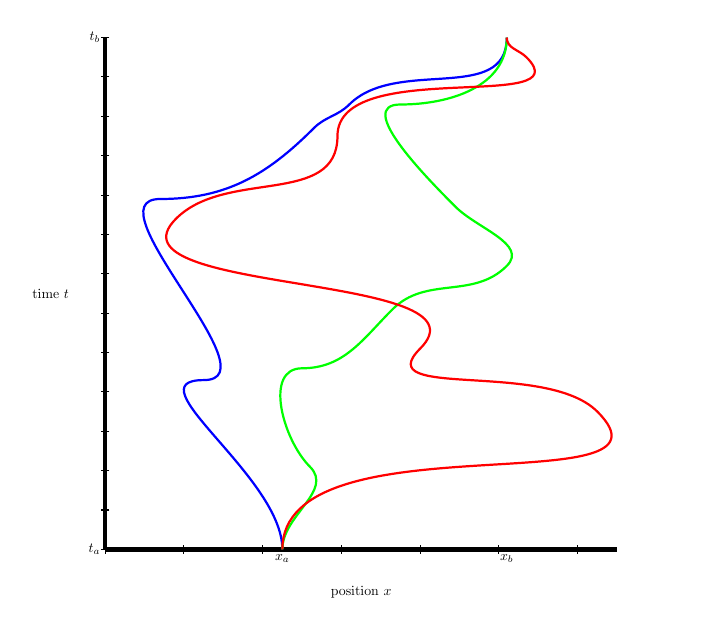
\begin{tikzpicture}[scale=0.5, every node/.style={transform shape}]
                \draw [ultra thick] [-] (0,13) -- coordinate (y axis mid) (0,0);
                \draw [ultra thick] [-] (0,0) -- coordinate (x axis mid) (13,0);
                \foreach \x in {0,2,...,13}
                    \draw (\x,3pt) -- (\x,-3pt);
                \foreach \y in {0,...,13}
                    \draw (3pt,\y) -- (-3pt,\y);
                \node[below=0.8cm] at (x axis mid) {position $x$};
                \node[left=0.8cm] at (y axis mid) {time $t$};
                \node [left] at (0,0) {$t_{a}$};
                \node [left] at (0,13) {$t_{b}$};
                \node [below] at (4.5,0) {$x_a$};
                \node [below] at (10.2,0) {$x_b$};
                \draw [-,thick, blue] (4.5,0) to [out=90,in=180] (2.5,4.3)
                        to [out=0,in=180] (1.4,8.9) to [out=0,in=-135] (5.3,10.7) 
                        to [out=45,in=225] (6.2,11.3) to [out=45,in=-90] (10.2,13);
                \draw [-,thick, green] (4.5,0) to [out=90,in=-45] (5.2,2.1)
                        to [out=135,in=180] (5.0,4.6) to [out=0,in=-135] (7.3,6.1) 
                        to [out=45,in=225] (10.2,7.2) to [out=45,in=-45] (8.9,8.7)
                        to [out=135,in=180] (7.5,11.3) to [out=0,in=-90] (10.2,13);
                \draw [-,thick, red] (4.5,0) to [out=90,in=-45] (12.5,3.5)
                        to [out=135,in=225] (8,5.1) to [out=45,in=-135] (1.8,8.4) 
                        to [out=45,in=270] (5.9,10.5) to [out=90,in=-45] (10.7,12.5)
                        to [out=135,in=-90] (10.2,13);
            \end{tikzpicture}
            \caption{Three of the infinitely many paths from $\left(x_a,t_a\right)$ to $\left(x_b,t_b\right)$ that contribute to the path integral.} 
            \label{fig:ExamplePathIntegrals}
        \end{figure}

        In the transition amplitude we integrate over an infinite number of paths, figure \ref{fig:ExamplePathIntegrals} shows three such paths that contribute to the path integral. The first step in calculating the path integral is to discretise time, this is shown in figure \ref{fig:TimeLattice} where we have discretised the green path in figure \ref{fig:ExamplePathIntegrals} onto a time lattice and we assume the particle travels along a straight line between the time sites.
        \begin{figure}
            \centering
            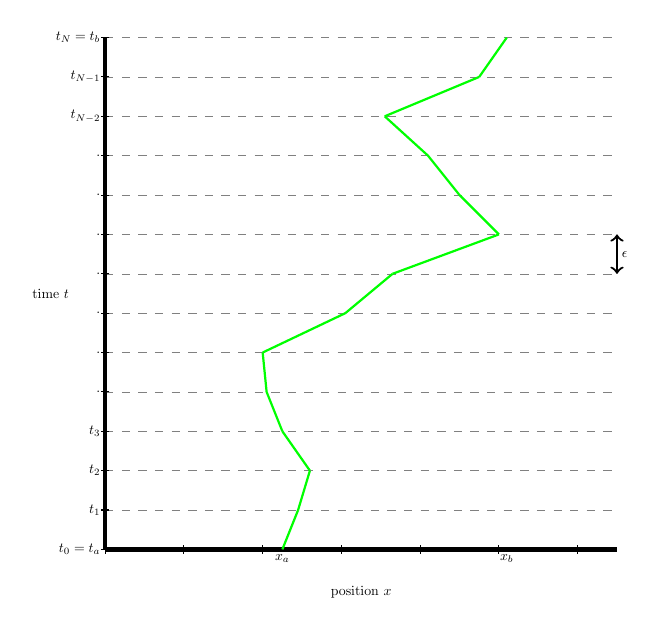
\begin{tikzpicture}[scale=0.5, every node/.style={transform shape}]
                
                \foreach \y in {0,...,13}{ \draw [help lines, dashed] (0,\y) -- (13,\y); }
                \draw [ultra thick] [-] (0,13) -- coordinate (y axis mid) (0,0);
                \draw [ultra thick] [-] (0,0) -- coordinate (x axis mid) (13,0);
                \foreach \x in {0,2,...,13}
                    \draw (\x,3pt) -- (\x,-3pt);
                \foreach \y in {0,...,13}
                    \draw (3pt,\y) -- (-3pt,\y);
                \node [left] at (0,0) {$t_{0}=t_{a}$};
                \node [left] at (0,1) {$t_{1}$};
                \node [left] at (0,2) {$t_{2}$};
                \node [left] at (0,3) {$t_{3}$};
                \node [left] at (0,4) {$.$};
                \node [left] at (0,5) {$.$};
                \node [left] at (0,6) {$.$};
                \node [left] at (0,7) {$.$};
                \node [left] at (0,8) {$.$};
                \node [left] at (0,9) {$.$};
                \node [left] at (0,10) {$.$};
                \node [left] at (0,11) {$t_{N-2}$};
                \node [left] at (0,12) {$t_{N-1}$};
                \node [left] at (0,13) {$t_{N}=t_{b}$};
                \node[below=0.8cm] at (x axis mid) {position $x$};
                \node[left=0.8cm] at (y axis mid) {time $t$};
                \draw [thick] [<->] (13,7) -- (13,8) ;
                \node [below=0.5cm] [right] at (13,8) {$\epsilon$};
                \draw [thick,green] (4.5,0) -- (4.9,1);
                \draw [thick,green] (4.9,1) -- (5.2,2);
                \draw [thick,green] (5.2,2) -- (4.5,3);
                \draw [thick,green] (4.5,3) -- (4.1,4);
                \draw [thick,green] (4.1,4) -- (4.0,5);
                \draw [thick,green] (4.0,5) -- (6.1,6);
                \draw [thick,green] (6.1,6) -- (7.3,7);
                \draw [thick,green] (7.3,7) -- (10,8);
                \draw [thick,green] (10,8) -- (9.0,9);
                \draw [thick,green] (9.0,9) -- (8.2,10);
                \draw [thick,green] (8.2,10) -- (7.1,11);
                \draw [thick,green] (7.1,11) -- (9.5,12);
                \draw [thick,green] (9.5,12) -- (10.2,13);
                \node [below] at (4.5,0) {$x_a$};
                \node [below] at (10.2,0) {$x_b$};
            \end{tikzpicture}
            \caption{Discretising time and a path from $\left(x_a,t_a\right)$ to $\left(x_b,t_b\right)$  onto a lattice of time spacing $\epsilon$.}
            \label{fig:TimeLattice}
        \end{figure}
        For each time site on the lattice $t_i$ we have a position $x_i = x\left(t_i\right)$ where $i=0,1,\dots,N$. We introduce the notation:
        \begin{equation}
            \label{eq:configuration}
            \bm{x}=\left(x_0,x_1,\dots,x_{N}\right)
        \end{equation}
        to denote a particular path on the lattice where each position coordinate has been specified and we refer to equation \ref{eq:configuration} as a \textit{configuration} on the lattice. In our notation for the labelling of the position eigenstates in equation \ref{eq:PathIntegral} we also have $x_b=x_{N}=x\left(t_{N}\right)$ and $x_a=x_0=x\left(t_0\right)$ in order to match with figure \ref{fig:TimeLattice}. $ \epsilon $ is the spacing between lattice sites and so $\epsilon = \frac{t_b-t_a}{N} = t_{i+1}-t_i$ and for $k=0,1,\dots,N$ we have $ t_k = t_a + k \epsilon $. In order to discretise the action in equation \ref{eq:MinkowskiAction} we approximate the derivative by a forward difference and the integral as a Riemann sum since we assume the particle is travelling on a straight line between lattice sites:
        
        \begin{equation}
            \label{eq:DiscreteMinkowskiAction}
            S_{M}\left(\bm{x}\right) = \sum_{i=0}^{N-1} \epsilon \left[\frac{1}{2}m\left(\frac{x_{i+1}-x_{i}}{\epsilon}\right)^{2} - V\left(x_i\right)\right].
        \end{equation}
        Since  for $i=1,2,\dots,N-1, -\infty < x_i < \infty$ we may define the integral measure in equation \ref{eq:PathIntegral} as:
        \begin{equation}
            \label{eq:IntegralMeasure}
            \int_{x_a}^{x_b} {\cal D} x \sim \prod_{n=1}^{N-1}\int_{-\infty}^{\infty}dx_n,
        \end{equation}
        which up to normalisation integrates over all possible routes through the lattice; so that for our discrete time lattice, the path integral is given by:
        \begin{equation}
            \label{eq:DiscretePathIntegral}
            Z_{ba} \sim \int^{+\infty}_{-\infty}\prod_{i=1}^{N-1}dx_i \exp{\left(\frac{i}{\hbar}S_M\left(\left\{x_i\right\}\right)\right)}.
        \end{equation}
        In the limit that $N\rightarrow \infty$ (or equivalently $\epsilon \rightarrow 0$) we recover (up to normalisation) equation \ref{eq:PathIntegral} from equation \ref{eq:DiscretePathIntegral} exactly. 

        We will impose periodic boundary conditions by identifying the first and last lattice sites (i.e. take $x_b=x_a$) and then integrate over that site, which can be quantified through: 
        \begin{align}
            Z & = \int dx_a \int dx_b \delta\left(x_b-x_a\right)Z_{ba} \\
              & \sim \int^{+\infty}_{-\infty}\prod_{i=0}^{N-1}dx_i \exp{\left(\frac{i}{\hbar}S_M\left\{x_i\right\}\right)}.
        \end{align}

        In order to work with the discrete path integral we have one final step. We make a \textit{Wick rotation} into imaginary time; this is done via the substitution:
        \begin{equation}
            \label{eq:WickRotation}
            \tau = it.
        \end{equation}
        Applying this to the discretised theory developed above by defining $a=i\epsilon$, we now have a lattice in imaginary time, of lattice spacing $a$, substituting $a$ into equation \ref{eq:DiscreteMinkowskiAction}:
        \begin{align}
            \label{eq:DiscreteEuclideanAction1}
            S_M\left(\bm{x}\right) & = i\sum_{i=0}^{N-1} a \left[\frac{1}{2}m\left(\frac{x_{i+1}-x_{i}}{a}\right)^2 + V(x_i)\right] \\
            \label{eq:DiscreteEuclideanAction2} & = iS_E\left(\bm{x}\right),
        \end{align}
        where we have redefined the notation slightly so that $x_i=x\left(\tau_i\right)$ since we now have a lattice in imaginary time.
        The quantity
        \begin{equation}
            \label{eq:DiscreteEuclideanAction}
            S_{E}\left(\bm{x}\right) \equiv \sum_{i=0}^{N-1} a \left[\frac{1}{2}m\left(\frac{x_{i+1}-x_{i}}{a}\right)^2 + V(x_i)\right]
        \end{equation}
        is the discretised ``Euclidean'' action; it has this name because the effect of the Wick transformation is that it turns the Minkowski metric $ds_{M}$ on the coordinates $\left(x,y,z,t\right)$ into the Euclidean metric $ds_{E}$ on the coordinates $\left(x,y,z,\tau\right)$ and vice-versa:
        \begin{align}
            \label{eq:MinkowskiMetric} ds_{M}^{2} & = -dt^2 + dx^2 + dy^2 + dz^2 \\
            \label{eq:MetricTransform}            & = d\tau^2 + dx^2 + dy^2 + dz^2 \\
            \label{eq:EuclideanMetric}            & = ds_{E}^{2}.
        \end{align}
        Equation \ref{eq:DiscreteEuclideanAction2} is a very useful result since upon substitution into the discrete path integral we find:
        \begin{equation}
            \label{eq:DiscreteEuclideanPathIntegral}
            Z \sim \int^{+\infty}_{-\infty}\prod_{i=0}^{N-1}dx_i \exp{\left(-\frac{1}{\hbar}S_{E}\left(\left\{x_i\right\}\right)\right)}
        \end{equation}
        which is known as the discrete euclidean path integral and will converge since the integrand is now exponentially suppressed. We have the standard result from statistical physics that for a system with a fixed number $N$ of continuous degrees of freedom labelled by $x_i$ for $i=0,1,\dots N-1$ then the canonical partition function is given by:
        \begin{equation}
            \label{eq:PartitionFunction}
            \mathcal{Z} \sim \int_{-\infty}^{+\infty}\prod_{i=0}^{N-1}dx_{i}\exp{\left(-\beta H\left(\left\{x_i\right\}\right)\right)},
        \end{equation}
        with $\beta=\frac{1}{k_{B}T}$ where $T$ is the system temperature and $k_{B}$ is the Boltzmann constant. Comparing equation \ref{eq:DiscreteEuclideanPathIntegral} to equation \ref{eq:PartitionFunction} we can see that the discretise Euclidean path integral is a classical canonical partition function on a system with $N$ degrees of freedom, provided that we take:
        \begin{equation}
            \label{ActionToHamiltonian}
            \frac{1}{\hbar}S_{E}\left(\left\{x_{i}\right\}\right) = \beta H\left(\left\{x_{i}\right\}\right).
        \end{equation}
        
        We then have a Boltzmann factor given by $\exp{\left(-\frac{1}{\hbar}S_{E}\left(\left\{x_{i}\right\}\right)\right)}$. So in summary we now have a classical interpretation of our quantum calculation of the path integral; our lattice is essentially a one dimensional crystal of size $N$ at temperature $T$ with a continuous variable $x_i$ at each crystal site, and its Hamiltonian is given by $S_E\left(\left\{x_i\right\}\right)$.

        It is interesting to note that in quantum mechanics, due to the uncertainty principle $\Delta x\Delta p \geq \frac{\hbar}{2}$, $\hbar$ provides a measure of quantum fluctuations in our system. As $\hbar \rightarrow 0$ we recover classical physics and in this limit the only path in the path integral that contributes to the transition amplitude is the classical one. On the other hand, in statistical mechanics $T$ provides a measure of statistical fluctuations in our system, and in the limit that $T \rightarrow 0$ these fluctuations go to zero. Hence taking the limit that $\hbar \rightarrow 0$ and $T \rightarrow 0$ we see statistical mechanics on a (real) crystal lattice is equivalent quantum mechanics in imaginary time.



\section{Methods}
    \subsection{Monte Carlo Methods}
    Monte Carlo methods provide a way of numerically evaluating integrals where the error is independent of the dimensionality of the integral. The general idea is that we can approximate the value of an $d$ dimensional integral:
    \begin{equation}
        I = \int_V d^{d}x f\left(\bm{x}\right)
    \end{equation}
    by considering it as an average value of the function over the integral volume:
    \begin{equation}
        I \approx \frac{1}{N}\sum_i^{N}f\left(\bm{x}_i\right),
    \end{equation}
    where $\bm{x}_i\in V$ are \textit{samples} from the integration domain. The most naive method for generating the samples is to draw them from a uniform distribution over the domain. To see why uniform sampling is naive note that the error in the Monte Carlo estimate on the integral is:
    \begin{align}
        \sigma_I \approx \frac{\sigma_f}{\sqrt{N}} = \sqrt{\frac{1}{N}\left[\frac{1}{N}\sum_{i=1}^{N}f\left(\bm{x}_i\right)^2-\left(\frac{1}{N}\sum_{i=1}^{N}f\left(\bm{x}_i\right)\right)^2\right]},
    \end{align}
    so that unless the function is very smooth and hence has a small variance, it will have a large error. It is equally likely that samples are taken from the subsets of the domain where $f\left(\bm{x}_i\right)$ is very small as when it is large, hence the integral converges very slowly. A solution to this problem is to use importance sampling. In importance sampling, rather than sample uniformly from the domain, samples are selected according to a probability distribution that gives preference to samples that give dominant contributions to the integral. To realise importance sampling we 
    \subsection{Hybrid Monte Carlo}
        \subsubsection{Hamiltonian Dynamics}
            \label{sec:HamiltonianDynamics}
            Due to the fundamental importance of Hamiltonian dynamics in the Hybrid-Monte-Carlo algorithm in this section we provide a quick review of Hamilton's equations and explain the numerical method used to integrate these equations so that they may be used in computational simulations.

            Hamiltonian Dynamics enables us to solve the time evolution of a system of canonical coordinates $\left(\bm{q},\bm{p}\right)$ where the $d$-dimensional $\bm{q}=\left(q_1,q_2,\dots,q_d\right)$ and $\bm{p}=\left(p_1,p_2,\dots,p_d\right)$ vectors are called \textit{position} and \textit{momentum} respectively. The system is then characterised by a Hamiltonian function $H\left(\bm{q},\bm{p}\right)$ on the $2d$-dimensional \textit{phase space} occupied by the $\left(\bm{q},\bm{p}\right)$ vectors. \textbf{Hamilton's equations}:
            \begin{align}
                \label{eq:HamiltonsEquation1} \frac{dq_i}{dt} & = \frac{\partial H}{\partial p_i} \\
                \label{eq:HamiltonsEquation2} \frac{dp_i}{dt} & = -\frac{\partial H}{\partial q_i}
            \end{align}
            for $i = 1, 2, \dots d$, provide the time evolution of the vectors $\bm{q}$ and $\bm{p}$. We will see in section \ref{sec:SamplingAndTheHamiltonian} for the purposes of the implementing the HMC algorithm we may assume that the Hamiltonian is of the form:
            \begin{equation}
                \label{eq:HamiltonianUPlusK}
                H\left(\bm{q},\bm{p}\right) = U\left(\bm{q}\right) + K\left(\bm{p}\right),
            \end{equation}
            Where $U\left(\bm{q}\right)$ and $K\left(\bm{p}\right)$ are known as the \textit{potential} and \textit{kinetic} terms respectively. Equations \ref{eq:HamiltonsEquation1} and \ref{eq:HamiltonsEquation2} then become:
            \begin{align}
                \label{eq:HamiltonsEquation1K} \frac{dq_i}{dt} & = \frac{\partial K}{\partial p_i} \\
                \label{eq:HamiltonsEquation2T} \frac{dp_i}{dt} & = -\frac{\partial U}{\partial q_i}.
            \end{align}

            Since we intend to use the solutions to Hamilton's equations in the HMC simulation we need to find a way of integrating them numerically; in Neal's review of Hamiltonian Monte-Carlo methods \cite{neal_2011} it is argued that a successful method for this is \textit{leapfrog integration}. In the leapfrog method to make the small time step $\epsilon$ from $t$ to $t+\epsilon$ on position and momentum we use the equations:
            \begin{align}
                \label{eq:LeapFrogEq1} p_i\left(t+\epsilon/2\right) & = p_i\left(t\right) + \epsilon/2\frac{dp_i}{dt}\left(t\right) = p_i\left(t\right) - \epsilon/2\frac{\partial U}{\partial q_i}\left(\bm{q}\left(t\right)\right), \\
                \label{eq:LeapFrogEq2}q_i\left(t+\epsilon\right) & = q_i\left(t\right) + \epsilon\frac{dq_i}{dt}\left(t+\epsilon/2\right) = q_i\left(t\right) + \epsilon\frac{\partial K}{\partial p_i}\left(\bm{p}\left(t+\epsilon/2\right)\right), \\
                \label{eq:LeapFrogEq3}p_i\left(t+\epsilon\right) & = p_i\left(t+\epsilon/2\right) + \epsilon/2\frac{dp_i}{dt}\left(t+\epsilon/2\right) = p_i\left(t+\epsilon/2\right) - \epsilon/2\frac{\partial U}{\partial q_i}\left(\bm{q}\left(t+\epsilon\right)\right),
            \end{align}
            where in the second equality in each step we have made the substitution for Hamilton's equations.
            In equation \ref{eq:LeapFrogEq1} we begin with a half step in each momentum component to go from $t$ to $t+\epsilon/2$. Using the half stepped momenta we then do a full step from $t$ to $t+\epsilon$ in each position component in equation \ref{eq:LeapFrogEq2}. We end in equation \ref{eq:LeapFrogEq3} with a second half step in the momentum components to go from $t+\epsilon/2$ to $t+\epsilon$ using the updated position components. Iterating this process we do as many steps of size $\epsilon$ as we like.

            This generalises to making $l$ steps in position and momentum and we can combine any two half steps in momentum that follow one another to simplify the algorithm which is often more convenient for computation purposes. Starting at $t=0$:
            \begin{enumerate}
                \item We begin with a half step in momentum:
                \begin{equation}
                    \label{eq:MomentumInitialHalfStep}
                    p_i\left(\epsilon/2\right) = p_i\left(0\right) - \epsilon/2\frac{\partial U}{\partial q_i}\left(\bm{q}\left(0\right)\right),
                \end{equation}
                and a full step in position:
                \begin{equation}
                    \label{eq:PositionInitialStep}
                    q_i\left(\epsilon\right) = q_i\left(0\right) + \epsilon\frac{\partial K}{\partial p_i}\left(\bm{p}\left(\epsilon/2\right)\right).
                \end{equation}
                \item Then make $l-1$ alternating steps in momentum and position:
                \begin{equation}
                    \label{eq:MomentumFullStep}
                    p_i\left(n\epsilon+\epsilon/2\right) = p_i\left(n\epsilon-\epsilon/2\right) - \epsilon\frac{\partial U}{\partial q_i}\left(\bm{q}\left(n\epsilon\right)\right),
                \end{equation}
                \begin{equation}
                    \label{eq:PositionFullStep}
                    q_i\left(n\epsilon+\epsilon\right) = q_i\left(n\epsilon\right) + \epsilon\frac{\partial K}{\partial p_i}\left(\bm{p}\left(n\epsilon+\epsilon/2\right)\right),
                \end{equation}
                for $n = 1, \dots , l-1$.
                \item Then a final half step in momentum:
                \begin{equation}
                    \label{eq:Momnetum}
                    p_i\left(l\epsilon\right) = p_i\left(l\epsilon-\epsilon/2\right) - \epsilon/2\frac{\partial U}{\partial q_i}\left(\bm{q}\left(l\epsilon\right)\right).
                \end{equation}
            \end{enumerate}
            The reasoning for the name \textit{leapfrog} becomes apparent here since apart from the initial and final half steps in momentum, the momentum and position values are used alternatively to calculate the position and momentum respectively at the next step and the variables ``leap'' over one another at on offset of $\epsilon/2$. 

            An important feature of the leap frog integration scheme that makes it applicable to HMC is that it preserves volume in phase space exactly, which we will see leads to detailed balance. For Hamiltonian dynamics in continuous time, preservation of volume in phase space is known as Louville's theorem and its proof is given by Goldstein, Poole and Safko's in \cite{goldstein_poole_safko_2014}. For the discrete dynamics integrated via the leap frog scheme we can easily verify that volume preservation is still the case. The leap frog equations \ref{eq:LeapFrogEq1}, \ref{eq:LeapFrogEq2} and \ref{eq:LeapFrogEq3} which evolve the system a single step in time from $t$ to $t+\epsilon$ can be rewritten using matrices as:
            \begin{align}
                \label{eq:leapfrogmatrix1}\begin{bmatrix} \bm{q}\left(t\right) \\ \bm{p}\left(t+\epsilon/2\right) \end{bmatrix} & =
                \begin{bmatrix} I_{d\times d} & 0_{d\times d} \\ A & I_{d\times d} \end{bmatrix}\begin{bmatrix} \bm{q}\left(t\right) \\ \bm{p}\left(t\right) \end{bmatrix} \\
                \label{eq:leapfrogmatrix2}\begin{bmatrix} \bm{q}\left(t+\epsilon\right) \\ \bm{p}\left(t+\epsilon/2\right) \end{bmatrix} & = 
                \begin{bmatrix} I_{d\times d} & \epsilon \\ 0_{d\times d} & I_{d\times d} \end{bmatrix} \begin{bmatrix} \bm{q}\left(t\right) \\ \bm{p}\left(t+\epsilon/2\right) \end{bmatrix} \\
                \label{eq:leapfrogmatrix3}\begin{bmatrix} \bm{q}\left(t+\epsilon\right) \\ \bm{p}\left(t+\epsilon\right) \end{bmatrix} & = 
                \begin{bmatrix} I_{d\times d} & 0_{d\times d} \\ B & I_{d\times d} \end{bmatrix} \begin{bmatrix} \bm{q}\left(t+\epsilon\right) \\ \bm{p}\left(t+\epsilon/2\right) \end{bmatrix}
            \end{align}
            where the off diagonal $d\times d$ matrices $A$ and $B$ are determined by the partial derivatives of the potential evaluated at $t$ and $t+\epsilon$ respectively. The form of $A$ and $B$ is not important here since the other off diagonal term is always a zero matrix (the transformation is always a sheer) so these elements make no contribution to the determinant which we will see below leads to preservation of volume. Combing equations \ref{eq:leapfrogmatrix1}, \ref{eq:leapfrogmatrix2} and \ref{eq:leapfrogmatrix3} we have that:
            \begin{equation}
                \label{eq:LeapFrogJacobian}
                \begin{bmatrix} \bm{q}\left(t+\epsilon\right) \\ \bm{p}\left(t+\epsilon\right) \end{bmatrix} =
                T \begin{bmatrix} \bm{q}\left(t\right) \\ \bm{p}\left(t\right) \end{bmatrix}
            \end{equation}
            where the $2d\times2d$ matrix $T$ is the Jacobian matrix of the transformation from $\left(\bm{q}\left(t\right),\bm{p}\left(t\right)\right)$ to $\left(\bm{q}\left(t+\epsilon\right),\bm{p}\left(t+\epsilon\right)\right)$ given by:
            \begin{equation}
                T= \begin{bmatrix} I_{d\times d} & 0_{d\times d} \\ A & I_{d\times d} \end{bmatrix} \begin{bmatrix} I_{d\times d} & \epsilon \\ 0_{d\times d} & I_{d\times d} \end{bmatrix} \begin{bmatrix} I_{d\times d} & 0_{d\times d} \\ B & I_{d\times d} \end{bmatrix}
            \end{equation}
            from which it is clear that $\text{det}\left(T\right)=1$ and therefore we have preservation of volume in phase space for a single step of the leap frog method. Clearly if volume is preserved for a single step it must be preserved for an arbitrary number of steps as well. We will return to this argument in section \ref{sec:Tempering} where we will show that the leap frog integration scheme preserves volume even for the case of tempered dynamics. 

            It is also obvious that the leapfrog integration scheme provides reversible dynamics; by negating the momenta at the end of a trajectory and applying the equations a second time we will return to the initial point in phase space. 

        

        \subsubsection{Sampling and the Hamiltonian}
            \label{sec:SamplingAndTheHamiltonian}
            For a physical system in thermodynamic equilibrium with a fixed number of degrees of freedom and with energy function $E\left(\bm{x}\right)$, where the vector $\bm{x} = \left(x_{1},x_{2},\dots,x_{d}\right)$ denotes the state of the system that depends on $d$ variables, the canonical Boltzmann distribution (probability density function for the states of the system) is given by:
            \begin{equation}
                \label{eq:BoltzmannDistribution}
                P\left(\bm{x}\right) = \frac{1}{Z} \exp{\left(-\frac{E\left(\bm{x}\right)}{T} \right)},
            \end{equation}
            where $Z$ is the canonical partition function for the system which provides the normalisation and is given by 
            \begin{equation}
                \label{eq:JointPartitionFunction}
                Z = \int\prod_{i=1}^{d}dx_{i} \exp{\left(-\frac{E\left(\bm{x}\right)}{T} \right)}.
            \end{equation}
            Alternatively any probability distribution $P\left(\bm{x}\right)$ can be constructed as the Boltzmann distribution for the energy function $ E\left(\bm{x}\right) = -T\left(\log{P\left(\bm{x}\right)} + \log{Z}\right)$ for some choice of $T$ and $Z$. 

            A Hamiltonian of the form $H\left(\bm{q},\bm{p}\right)=U\left(\bm{q}\right)+K\left(\bm{p}\right)$ is an energy function on the $2d$-dimensional phase space given by position and momentum $\left(\bm{q},\bm{p}\right)$, with $\bm{q} = \left(q_{1},q_{2},\dots,q_{d}\right)$ and $\bm{p} = \left(p_{1},p_{2},\dots,p_{d}\right)$. We may define a Boltzmann distribution on those variables by:
            \begin{equation}
                \label{eq:BoltzmannDistributionXP}
                P\left(\bm{q},\bm{p}\right) = \frac{1}{Z}\exp{\left(-\frac{H\left(\bm{q},\bm{p}\right)}{T} \right)},
            \end{equation}
            with 
            \begin{equation}
                Z = \int\prod_{i=1}^{d}dx_{i}dp_{i} \exp{\left(\frac{-H\left(\bm{q},\bm{p}\right)}{T}\right)}
            \end{equation}
            Then, if $H\left(\bm{q},\bm{p}\right) = U\left(\bm{q}\right) + K\left(\bm{p}\right)$ this factorises as:
            \begin{equation}
                \label{eq:BoltzmannDistributionXPFactorised}
                P\left(\bm{q},\bm{p}\right) = \frac{1}{Z_U}\exp{\left(-\frac{U\left(\bm{q}\right)}{T} \right)}\frac{1}{Z_K}\exp{\left(-\frac{K\left(\bm{p}\right)}{T} \right)} = P\left(\bm{q}\right) P\left(\bm{p}\right),
            \end{equation}
            so the variables $\bm{q}$ and $\bm{p}$ and their respective probability distributions are independent. This means that in order to sample $\bm{q}$ from the marginal distribution $P\left(\bm{q}\right)$ we can sample from the joint distribution $P\left(\bm{q},\bm{p}\right)$ and disregard the $\bm{p}$. 

            In the HMC algorithm we employ Hamiltonian dynamics to sample from the joint distribution $P\left(\bm{q},\bm{p}\right)$. Therefore, if we have some probability distribution $P\left(\bm{x}\right)$ for states $\bm{x}$ we wish to sample, we may through equation \ref{eq:BoltzmannDistribution} define an energy function $E\left(\bm{x}\right)$ for that distribution. We then define $\bm{q}\equiv\bm{x}$ and $U\left(\bm{q}\right) \equiv E\left(\bm{x}\right)$, introduce ``fictitious momenta'' $\bm{p}$ and define a kinetic energy $K\left(\bm{p}\right)$ and the Hamiltonian $H\left(\bm{q},\bm{p}\right) = U\left(\bm{q}\right) + K\left(\bm{p}\right)$. Running the HMC algorithm generates samples according to the distribution given by equation \ref{eq:BoltzmannDistributionXP}, but by the factorization in equation \ref{eq:BoltzmannDistributionXPFactorised} this gives samples of $\bm{x}$ according to out original distribution $P\left(\bm{x}\right)$. In the HMC algorithm, we think of the variables of interest $\bm{x}$ as position $\bm{q}$ with conjugate momenta $\bm{p}$ which of course matches up nicely in physical applications where we are actually sampling position, although the algorithm is equally applicable in non-physical cases.

            Since the fictitious momenta $\bm{p}$ are introduced artificially, we need to choose their probability distribution $P\left(\bm{p}\right)$ by specifying the kinetic energy function $K\left(\bm{p}\right)$. For the purposes of our work we may take:
            \begin{equation}
                \label{eq:HMCQuadraticKineticEnergy}
                K\left(\bm{p}\right) = \sum_{i=1}^{d}\frac{p_i^2}{2}
            \end{equation}
            and $T=1$ from now on.

            \subsubsection{Steps of the HMC Algorithm}
            Here we will outline the main steps of the HMC algorithm then give a more detailed explanation of each stage and its implementation.
            \begin{enumerate}
                \setcounter{enumi}{-1}
                \item \label{en:HMCStep0} Provide an initial sample $\bm{q}$
                \item \label{en:HMCStep1} Generate $\bm{p}$ from the multivariate Gaussian Distribution $\mathcal{N}\left(\bm{0},I_{d\times d}\right)$ 
                \item \label{en:HMCStep2} Evolve the variables from $\left(\bm{q},\bm{p}\right)$ to $\left(\bm{q^{*}},\bm{p^{*}}\right)$ using Hamilton's equations of motion.
                \item \label{en:HMCStep3} Accept the proposed state $\left(\bm{q^{*}},\bm{p^{*}}\right)$ with probability:
                        \begin{equation*}
                            \min{\left[1,\exp{\left(-H_{HMC}\left(\bm{q}^{*},\bm{p}^{*}\right)+ \allowbreak H_{HMC}\left(\bm{q},\bm{p}\right)\right)}\right]}
                        \end{equation*}
                        If proposed state rejected, record current state $\bm{q}$ as sample (i.e. state started with), if successful set current state to proposed state $\bm{q}$ = $\bm{q^{*}}$ and record it as a sample.
                \item \label{en:HMCStep5} Return to step \ref{en:HMCStep1} with $\bm{q}$.
            \end{enumerate}

            In step \ref{en:HMCStep0} we provide an initial state. This can be chosen or generated randomly; some starting configurations are better than others\todo{Good place for a reference}. However, since we normally disregard the samples generated in the early HMC iterations (see section \todo{Reference section on thermalization}) this choice is not critical. 

            In step \ref{en:HMCStep1} we draw the fictitious momenta according to their probability distribution. The choice of kinetic energy in equation \ref{eq:HMCQuadraticKineticEnergy} and the form of equation \ref{eq:BoltzmannDistribution} means that:
            \begin{align}
                \label{eq:KineticBoltzmannDistribution}
                P\left(\bm{p}\right) & = \frac{1}{Z_K}\exp{\left(-\sum_{i=1}^{d}\frac{p_i^2}{2}\right)} \\
                                     & = \frac{1}{Z_K} \prod_{i}^{d}\exp{\left(-\frac{p_i^2}{2}\right)}
            \end{align}
            and
            \begin{align}
                Z_k & = \int \prod_{i=1}^{d} dp_i \exp{\left(-\frac{1}{2}\sum_{i=1}^{d}p_i^2\right)} \\
                    & = \int \prod_{i=1}^{d} dp_i \prod_{i=1}^{d} \exp{\left(-\frac{p_i}{2}\right)} \\
                    & = \prod_{i=1}^{d}Z_{K_i}
            \end{align}
            such that
            \begin{equation}
                Z_{K_i} = \int dp_i \exp{\left(-\frac{1}{2}p_i\right)} = \sqrt{2\pi}.
            \end{equation}
            We can then see that the canonical distribution function for the momentum factorises into the marginal distribution functions, that is:
            \begin{equation}
                P\left(\bm{p}\right) = \prod_{i=1}^{d} \frac{1}{Z_{K_i}}P\left(p_i\right)
            \end{equation}
            where each marginal distribution $P\left(p_i\right)$ is given by:
            \begin{equation}
                \label{eq:KineticMarginalDistribution}
                P\left(p_{i}\right) = \frac{1}{Z_{k_i}}\exp{\left(-\frac{p_i^2}{2}\right)} = \frac{1}{\sqrt{2\pi}} \exp{\left(-\frac{p_i^2}{2}\right)}
            \end{equation}
            which is a Gaussian distribution of mean $0$ and variance $1$. Each component $p_i$ of $\bm{p}$ is therefore drawn from a Gaussian $\mathcal{N}{\left(0,1\right)}$, so we draw $\bm{p}$ from a multivariate Gaussian distribution of mean $\bm{0}$ and covariance $I_{d\times d}$ .

            In step \ref{en:HMCStep2} we evolve the variables $\left(\bm{q},\bm{p}\right)$ by integrating Hamilton's equations. In order to implement this in a computer simulation we use the leapfrog method described in section \ref{sec:HamiltonianDynamics}. We have a choice of the number of time steps $l$ and their size $\epsilon$; it is common practice in HMC to choose $\epsilon$ and $l$ such that $l\epsilon=1$.


            In step \ref{en:HMCStep3} we accept or reject the proposed state with a probability given by:
            \begin{equation}
                \label{eq:HMCMetropolisUpdate}
                P\left(\bm{q}^{*},\bm{p}^{*},\bm{q},\bm{p}\right) = \min{\left[1,\exp{\left(-H_{HMC}\left(\bm{q}^{*},\bm{p}^{*}\right)+ \allowbreak H_{HMC}\left(\bm{q},\bm{p}\right)\right)}\right]},
            \end{equation}
            which is known as a \textit{Metropolis update}. The interpretation of \ref{eq:HMCMetropolisUpdate} is that if the Hamiltonian decreases (or stays constant) as a result of moving to the proposed state the update is accepted with certainty. However, if the Hamiltonian increases as a result of the moving to the proposed state, the proposal is accepted with a probability that decreases for larger increases in the Hamiltonian. If the state is accepted then it becomes the current state state i.e. $\bm{q} = \bm{q^*}$, otherwise the current state remains as it was in step \ref{en:HMCStep1}. In either case we then record the current state as a sample and return to step \ref{en:HMCStep1} with the current state $\bm{q}$.

            From the Metropolis update in equation \ref{eq:HMCMetropolisUpdate} we can show that for smaller value of $\epsilon$ and larger $l$ (i.e. smaller time steps and more of them) the probability of accepting an update approaches unity. To see this note that as $\epsilon \rightarrow 0$ and $l \rightarrow \infty$ the leap frog method approaches an exact integration of Hamilton's equations. It is easily shown that for continuous time the Hamiltonian is a conserved quantity:
            \begin{align}
            \frac{dH}{dt}=\sum_{i=1}^{d}\left[\frac{dq_i}{dt}\frac{\partial H}{\partial q_i}+\frac{dp_i}{dt}\frac{\partial H}{\partial p_i}\right]=\sum_{i=1}^{d}\left[\frac{\partial H}{\partial p_i}\frac{\partial H}{\partial q_i}-\frac{\partial H}{\partial q_i}\frac{\partial H}{\partial p_i}\right]=0
            \end{align}
            where in the second equality we have used Hamilton's equations. Therefore as $\epsilon \rightarrow 0$ and $l\rightarrow \infty$, $H_{HMC}\left(\bm{q},\bm{p}\right) \rightarrow H_{HMC}\left(\bm{q}^*,\bm{p}^*\right)$ and so the probability of accepting a state is always unity.   

            As $\epsilon$ decreases $l$ increases provided $l\epsilon$ is kept fixed, therefore more steps and hence a larger computational cost is required for proposal states with smaller $\epsilon$ in the trajectory. Conversely if we have a fixed computation time, then for smaller $\epsilon$ we will generate less proposals with a higher acceptance rate and hence our the error in the Monte-Carlo estimate on any observable will be larger. It is shown by Beskos et al. in \cite{beskos_pillai_roberts_sanz-serna_stuart_2013} that an acceptance rate of $\sim 65.1\%$ provides an optimal balance between the cost of generating proposals and the total number of samples.
          

            

            
\section{Results and Discussion}
    \subsection{Quantum Oscillators}
    In section \ref{sec:QuantumMechanics} we showed in equation \ref{eq:DiscreteEuclideanPathIntegral} that by discretising the path integral and performing a Wick rotation into imaginary time the path integral of quantum mechanics is a partition function if $S_E\left(\left\{x_i\right\}\right)= H\left(x_i\right)$ (working now in units where $\hbar=T=k_B=1$). The Hamiltonian is an energy function of the system and so we may use equation \ref{eq:BoltzmannDistribution} with $E\left(\bm{x}\right) = S_E\left(\bm{x}\right)$ to get the Boltzmann distribution:
    \begin{equation}
        \label{eq:BoltzmannDistributionPathIntegral}
        P\left(\bm{x}\right) = \frac{1}{Z}\exp{\left(-S_E\left(\bm{x}\right)\right)}.
    \end{equation}
    The probability distribution of equation \ref{eq:BoltzmannDistributionPathIntegral} is the distribution we wish to draw are samples according to for the Monte Carlo simulations, therefore we follow the method of section \ref{sec:SamplingAndTheHamiltonian} with this distribution, taking $\bm{q}\equiv\bm{x}$,
    \begin{align}
        \label{eq:QuantumHMCPotential}
        U\left(\bm{q}\right) & \equiv S_E\left(\bm{x}\right) \\
                             & = \sum_{i=0}^{N-1} a \left[\frac{1}{2}m\left(\frac{x_{i+1}-x_{i}}{a}\right)^2 + V(x_i)\right]
    \end{align} 
    and the kinetic energy $K\left(\bm{p}\right)$ as in equation \ref{eq:HMCQuadraticKineticEnergy}. We define our HMC Hamiltonian:
    \begin{align}
        \label{eq:HMCQuantumMechanicalHamiltonian1}
        H_{hmc}\left(\bm{q},\bm{p}\right) & \equiv K\left(\bm{p}\right) + U\left(\bm{q}\right)\\
        \label{eq:HMCQuantumMechanicalHamiltonian2} & = \sum_{i=0}^{N-1} \frac{p_i^2}{2} + S_E\left(\bm{q}\right) \\
        \label{eq:HMCQuantumMechanicalHamiltonian3}& = \sum_{i=0}^{N-1} \frac{p_i^2}{2} + \sum_{i=0}^{N-1} \epsilon \left[\frac{1}{2}m\left(\frac{q_{i+1}-q_{i}}{\epsilon}\right)^2 + V\left(q_i\right)\right],
    \end{align} 
    we can then use this Hamiltonian to generate samples with the HMC algorithm for any $1$-dimensional quantum mechanical system, by specifying the potential $V\left(x\right)$. With the choice of kinetic energy given in equation \ref{eq:HMCQuadraticKineticEnergy} and $U\left(\bm{q}\right) \equiv S_E\left(\bm{x}\right)$ this leads to the approximate solutions to Hamilton's equations in leapfrog implementation for $l$ steps of size $\epsilon$ taking the form:
            \begin{enumerate}
                \item Half step in momentum:
                \begin{equation}
                    \label{eq:MomentumInitialHalfStepQuadraticQHO}
                    p_i\left(\epsilon/2\right) = p_i\left(0\right) - \epsilon/2\left[\frac{m}{a}\left(2q_i\left(0\right)-q_{i-1}\left(0\right)-q_{i+1}\left(0\right)\right)+a\frac{\partial V\left(q_i\left(0\right)\right)}{\partial q_i}\right],
                \end{equation}
                full step in position:
                \begin{equation}
                    \label{eq:PositionInitialStepQuadraticQHO}
                    q_i\left(\epsilon\right) = q_i\left(0\right) + \epsilon p_i\left(\epsilon/2\right).
                \end{equation}
                \item Make $l-1$ alternating steps in momentum and position:
                \begin{equation}
                    \label{eq:MomentumFullStepQuadraticQHO}
                    p_i\left(n\epsilon+\epsilon/2\right) = p_i\left(n\epsilon-\epsilon/2\right) - \epsilon\left[\frac{m}{a}\left(2q_i\left(n\epsilon\right)-q_{i-1}\left(n\epsilon\right)-q_{i+1}\left(n\epsilon\right)\right)+a\frac{\partial V\left(q_i\left(n\epsilon\right)\right)}{\partial q_i}\right],
                \end{equation}
                \begin{equation}
                    \label{eq:PositionFullStepQuadraticQHO}
                    q_i\left(n\epsilon+\epsilon\right) = q_i\left(n\epsilon\right) + \epsilon p_i\left(n\epsilon+\epsilon/2\right),
                \end{equation}
                for $n = 1, \dots , l-1$.
                \item Final half step in momentum:
                \begin{equation}
                    \label{eq:MomnetumQuadraticKinetic}
                    p_i\left(\epsilon l\right) = p_i\left(l\epsilon-\epsilon/2\right) - \epsilon/2\left[\frac{m}{a}\left(2q_i\left(\epsilon l\right)-q_{i-1}\left(\epsilon l\right)-q_{i+1}\left(\epsilon l\right)\right)+a\frac{\partial V\left(q_i\left(\epsilon l\right)\right)}{\partial q_i}\right].
                \end{equation}
            \end{enumerate}
    
        \subsubsection{Quantum Harmonic Oscillator}
            \label{sec:QuantumHarmonicOscillator}
            We begin by applying the HMC algorithm to the quantum harmonic oscillator. Since this system has an analytic solution it is a good testing ground for checking our simulation is correct. The potential for the quantum harmonic oscillator can be parametrised as:
            \begin{equation}
                \label{eq:HarmonicPotential}
                V\left(x\right) = \frac{1}{2}\mu^2x^2
            \end{equation}
            where $\mu \in \mathbb{R}$.

            \paragraph{Typical Trajectory}
                Figure \ref{fig:TypicalHarmonicTrajectory} shows a typical path for the HMC simulation of the harmonic oscillator. This is just a plot of the position variable at each lattice site. 
                \begin{figure}
                    \centering
                        \begin{tikzpicture}[scale=1.5]
                            \begin{axis}[
                                xlabel= {$x$},
                                ylabel style ={rotate=0},
                                ylabel= {Lattice Site},
                                enlargelimits=true,
                                        ]
                                \addplot[color=black,mark=x,skip coords between index={100}{1000}]
                                table[x index=1, y index=0]{DataForReport/HarmonicTypicalTrajectory.dat};
                            \end{axis}
                        \end{tikzpicture}
                        \caption{Typical configuration for the harmonic oscillator with $\mu^2 = 1, m = 1, a = 1, L = 1000, d = 0.1, N = 10, \text{configurations} = 100000, \text{burn period} = 1000$.}
                        \label{fig:TypicalHarmonicTrajectory}
                \end{figure}
            \paragraph{Mean Square Position}
                The first quantity we calculate is the mean square position. For the discrete theory, the value this quantity for an imaginary time lattice of spacing $a$ and size $N$ can be calculated exactly to be: 
                \begin{equation}
                    \label{eq:MeanSquarePosition}
                    \braket{x^2} = \frac{1}{2\mu\left(m+\frac{a^2\mu^2}{4}\right)^\frac{1}{2}}\left(\frac{1+R^N}{1-R^N}\right),
                \end{equation}
                where
                \begin{equation}
                    \label{eq:R}
                    R = 1 + \frac{a^2\mu^2}{2m} - \frac{a\mu}{\sqrt{m}}\left( 1 + \frac{a^2\mu^2}{4m}\right)^{\frac{1}{2}},
                \end{equation}
                see \cite{creutz_freedman_1981} or appendix \ref{ap:DiscretePathIntegralDerivation} for a full derivation of equation \ref{eq:MeanSquarePosition}. Running the HMC simulation at a range of lattice spacings we obtain the results in figure \ref{fig:MeanXSquaredPlot}.
                \begin{figure}
                    \centering
                    \begin{tikzpicture}[scale=1.5]
                        \begin{axis}[
                            legend style={font=\tiny},
                            xlabel= {$a$},
                            ylabel style ={rotate=-90},
                            ylabel= {$\braket{x^2}$},
                            enlargelimits=true,
                                    ]
                            \addplot[only marks, 
                                   mark=x,color=black]
                                plot [error bars/.cd, 
                                    y dir = both, 
                                    y explicit]
                                table[x index=0, 
                                    y index=1, 
                                    y error index=2]{DataForReport/LatticeSpacingvsExpectationXSquared.dat};
                            \addlegendentry{Measured Values}
                            \addplot[domain=0:1,
                                samples=100,
                                color=blue,
                                    ]
                                {(1/2)*(1/sqrt(1+0.25*x*x)) * ((1+(1+0.5*x*x-x*sqrt(1+0.25*x*x))^(1000))/((1-(1+0.5*x*x-x*sqrt(1+0.25*x*x))^(1000))))};
                         \addlegendentry{Discrete Theory}      
                        \end{axis}
                    \end{tikzpicture}
                    \caption{Relationship between lattice spacing and expectation of position squared for the harmonic oscillator with $\mu^2 = 1, m = 1.$}
                    \label{fig:MeanXSquaredPlot}
                \end{figure}

            \paragraph{Energy Levels}
                In order to calculate the ground state energy of the system we use the virial theorem:
                \begin{equation}
                    \label{eq:VirialTheorem}
                    2\braket{\hat{T}} = \braket{xV'\left(x\right)}
                \end{equation}
                which relates the expectation value of kinetic energy to that of the potential and the derivation of which can be found in Binney and Skinner's The Physics of Quantum Mechanics \cite{binney_skinner_2015} and was orginally proved by Fock in \cite{fock_1930}. Applying this to the harmonic potential of equation \ref{eq:HarmonicPotential} we get:
                \begin{align}
                    \label{eq:HarmonicVirialTheorem}  E & = \braket{\hat{T}} +\braket{V\left(x\right)} \\
                                                        & = m\mu^2\braket{x^2},
                \end{align}
                so that for measurements made in the ground state:
                \begin{align}
                    \label{eq:HarmonicGroundStateEnergy}
                    E_0 = m\mu^2\braket{x^2}
                \end{align}
                Of course when $\mu=m=1$ the calculated values for the ground state energy are the same as those for $\braket{x^2}$ in figure \ref{fig:MeanXSquaredPlot}. When we recover the continuum limit as $a\rightarrow0$ and $N\rightarrow\infty$ we see that $E_0$ approaches the value of $\frac{1}{2}$ which is given by:
                \begin{equation}
                    \label{eq:ContinuumEnergyLevels}
                    E_n=\mu\left(n+\frac{1}{2}\right).
                \end{equation}
                To calculate the energy gap between the first and ground state we use:
                \begin{equation}
                    \label{eq:FirstExcitedStateHarmonicOscillator}
                    \Delta E\left(\delta \tau\right) = -\frac{1}{\delta \tau} \ln C\left(\delta \tau\right),
                \end{equation}
                where:
                \begin{equation}
                    \label{eq:CorrelationFunction}
                    C\left(\delta\tau\right) = \frac{\sum_{i=0}^{N-1} x_{i}x_{i+\delta\tau}}{\sum_{i=0}^{N-1}x_i^2}
                \end{equation}
                is the \textit{correlation function}. In equation \ref{eq:CorrelationFunction} we have utilized the periodic boundary conditions of the lattice and calculated the correlation at each lattice site then averaged over them to increase the statistics.\todo{Is this okay?} For an derivation of equation \ref{eq:FirstExcitedStateHarmonicOscillator} see appendix \todo{Insert reference to appendix.}
                Figures \ref{} and \ref{} show the energy gap and correlation function respectively on an HMC simulation of the harmonic oscillator.
                \begin{figure}
                    \centering
                    \begin{subfigure}[b]{0.4\textwidth}
                        \begin{tikzpicture}[scale=0.7]
                            \begin{axis}[
                                legend style={font=\tiny},
                                xlabel= {Lattice Site},
                                ylabel style ={rotate=0},
                                ylabel= {Correlation Function},
                                enlargelimits=true,
                                        ]
                                \addplot[only marks, 
                                       mark=x,color=black]
                                    plot [error bars/.cd, 
                                        y dir = both, 
                                        y explicit]
                                    table[x index=0, 
                                        y index=1, 
                                        y error index=2]{DataForReport/HarmonicCorrelationFunction.dat};
                            \end{axis}
                        \end{tikzpicture}
                        \caption{Correlation function.}
                        \label{fig:HarmonicCorrelationFunction}
                    \end{subfigure}
                    \begin{subfigure}[b]{0.4\textwidth}
                        \begin{tikzpicture}[scale=0.7]
                            \begin{axis}[
                                legend style={font=\tiny},
                                xlabel= {Lattice Time},
                                ylabel style ={rotate=0},
                                ylabel= {Energy Gap},
                                enlargelimits=true,
                                        ]
                                \addplot[only marks, 
                                       mark=x,color=black]
                                    plot [error bars/.cd, 
                                        y dir = both, 
                                        y explicit]
                                    table[x index=0, 
                                        y index=1, 
                                        y error index=2]{DataForReport/HarmonicCorrelationFunction.dat};
                            \end{axis}
                        \end{tikzpicture}
                        \caption{Energy gap}
                        \label{fig:HarmonicEnergyGap.}
                    \end{subfigure}
                    \caption{Energy gap and correlation function for the harmonic oscillator with $a=1$, $\mu=1$ and $m=1$.}
                    \label{fig:HarmonicEnergyGapAndCorrelatioFunction}
                \end{figure}
                For small values of $\delta \tau$ we can see that $\Delta E \approx 1$ which is what we expect from equation \ref{eq:ContinuumEnergyLevels}. \todo{Why doesn't it stay constant?} By averaging over the values for which $\Delta E \approx 1$ we can estimate the the first excited energies by subtracting the estimated ground state energy for various values of $\mu^2$. These have been plotted in figure \ref{} alongside the ground state energies for a selection of lattice spacings along with the results from the discrete and continuous theory.\todo{Make data for the plot and include the plot}
                \begin{figure}
                \centering
                \begin{tikzpicture}[scale=1.5]
                            \begin{axis}[
                                legend style={font=\tiny},
                                legend style={at={(0.03,0.5)},anchor=west},
                                xlabel= {Lattice Spaceing $a$},
                                ylabel style ={rotate=0},
                                ylabel= {Energy},
                                enlargelimits=true,
                                        ]
                                \addplot[only marks, 
                                       mark=x,color=black]
                                    plot [error bars/.cd, 
                                        y dir = both, 
                                        y explicit]
                                    table[x index=0, 
                                        y index=1, 
                                        y error index=2]{DataForReport/GroundAndFirstEnergies.dat};

                                \addplot[domain=0:1,
                                samples=100,
                                color=blue,
                                    ]
                                {(1/2)*(1/sqrt(1+0.25*x*x)) * ((1+(1+0.5*x*x-x*sqrt(1+0.25*x*x))^(1000))/((1-(1+0.5*x*x-x*sqrt(1+0.25*x*x))^(1000))))};
                                \addlegendentry{Ground State Discrete Theory}
                                \addplot[domain=0:1,
                                samples=100,
                                color=red,
                                    ]
                                {1.5*sqrt(1+0.25*x*x)};
                                \addlegendentry{First Excited State Discrete Theory}
                                \addplot[domain=0:1,
                                samples=100,
                                color=orange,
                                    ]
                                {0.5};
                                \addlegendentry{Ground State Continuum Theory}
                                \addplot[domain=0:1,
                                samples=100,
                                color=green,
                                    ]
                                {1.5};
                                \addlegendentry{First Excited State Continuum Theory}

                            \end{axis}
                        \end{tikzpicture}
                        

                \caption{Ground and first excited state energies for the HMC simulation with the continuum and discrete theory results.}
                \label{fig:HarmonicEnergyLevels}
                \end{figure}
                

            \paragraph{Ground State Wave Function}
            Our method for measuring the ground state wave function follows that of \cite{creutz_freedman_1981}. We discretise position into $K$ bins of size $\Delta x$. On any given configuration we may then bin the position coordinate at each lattice site and create a histogram. Normalising the histogram gives the probability mass density for finding the particle in any interval $x+\Delta x$ and as $\Delta x \rightarrow 0$, this becomes the probability density function that is the square amplitude of the wave function. On any configuration position coordinates are therefore binned according to:
                \begin{figure}
                    \centering
                    \begin{tikzpicture}[scale=1.5]
                        \begin{axis}[
                            legend style={font=\fontsize{4}{5}\selectfont},
                            xlabel= {$x$},
                            ylabel style ={rotate=-90},
                            ylabel= {$\left|\psi{\left(x \right)}\right|^2$},
                            enlargelimits=true,
                                    ]
                            \addplot[only marks, 
                                mark=x,color=black]
                                plot[error bars/.cd, 
                                    y dir = both, 
                                    y explicit]
                                table[x index=0, 
                                y index=1, 
                                y error index=2]{DataForReport/HarmonicWaveFunction.dat};
                            \addlegendentry{Measured Values}
                            \addplot[domain=-4:4,
                                samples=100,
                                color=blue,
                                    ]
                                {sqrt(sqrt(5)/(2*pi))*e^(-0.5*sqrt(5)*x*x)};
                            \addlegendentry{Discrete Theory}
                            \addplot[domain=-4:4,
                                samples=100,
                                color=red,
                                    ]
                                {1/sqrt(pi)*e^-x*x};
                            \addlegendentry{Continuum Theory}
                        \end{axis}
                    \end{tikzpicture}
                    \caption{Continuum, discrete and measured wave functions for the harmonic oscillator with $\mu^2 = 1, m = 1, a = 1, L = 1000, d = 0.1, N = 10, \text{configurations} = 100000, \text{burn period} = 1000$.}
                    \label{fig:HarmonicWaveFunction}
                \end{figure}


        \subsubsection{Quantum Anharmonic Oscillator}
            Since the anharmonic oscillator does not have an analytic solution for the properties we wish to calculate, it is a good first application of the Hybrid Monte Carlo method for calculations we do not already know the answer to. Rather than use the more common form of the anharmonic quartic potential:
            \begin{equation}
                \label{eq:AharmonicPotentialLambda}
                V\left(x\right) = \frac{1}{2}m\mu^2x^2+\lambda x^4
            \end{equation}
            where $\mu^2 \in\mathbb{R}$ and $\lambda\in\mathbb{R}_{>0}$, we use the potential:
            \begin{equation}
                \label{eq:AnharmonicPotentialF}
                V\left(x\right) = \lambda\left(x^2-f^2\right)
            \end{equation}
            with $\lambda\in\mathbb{R}_{>0}$ and $f^2\in\mathbb{R}_{>0}$. This form of the potential has the advantage that its zeros coincide with its minima at $x=\pm f$. Since potential \ref{eq:AnharmonicPotentialF} is equivalent to potential \ref{eq:AharmonicPotentialLambda} up to the additive constant $\lambda f^4$, the action and consequently the HMC Hamiltonian for the system is the same up to the additive constant $\lambda f^4$ also. This makes no difference to the measured quantities since the constant in the Hamiltonian vanishes when we take its derivatives in Hamilton's equations, and any constant term in the action amounts to rescaling the path integral in equation \ref{eq:PathIntegral} by a complex exponential factor, which will therefore vanish when we take the magnitude to get the probability.
            \paragraph{Typical Trajectory}
                Figure \ref{} shows a typical trajectory for the HMC simulation of the anharmonic oscillator. We can now observe the tunnelling behaviour we expect for a quantum system.
                \begin{figure}
                    \centering
                    \begin{tikzpicture}[scale=1.5]
                        \begin{axis}[
                            legend style={font=\tiny},
                            xlabel= {$x$},
                            ylabel style ={rotate=0},
                            ylabel= {Lattice Site},
                            enlargelimits=true,
                                    ]
                            \addplot[color=black,mark=x,skip coords between index={100}{1000}]
                            table[x index=1, y index=0]{DataForReport/AnharmonicTypicalTrajectory.dat};
                            
                            \draw [blue,dashed] (axis cs: -2,-10) -- (axis cs: -2,110);
                            \draw [blue,dashed] (axis cs: 2,-10) -- (axis cs:2,110);
                        \end{axis}
                    \end{tikzpicture}
                    \caption{Typical configuration for the anharmonic oscillator with $\lambda = 1, f^2 = 4, m = 1, a = 1, L = 1000, d = 0.01, N = 100, \text{configurations} = 100000, \text{burn period} = 1000$.}
                    \label{fig:TypicalAnharmonicTrajectory}
                \end{figure}
            \paragraph{Energy Levels}
                In order to calculate the ground state energy we proceed with the same method we used in the case of the harmonic oscillator in section \ref{sec:QuantumHarmonicOscillator} and use the virial theorem of equation \ref{eq:VirialTheorem} which gives:
                \begin{equation}
                    \label{eq:VirialTheoremAnharmonicOsillator}
                    E_0=3\lambda\braket{x^4}-4\lambda f^2\braket{x^2}+\lambda f^4.
                \end{equation}
                To calculate the first excited state we\todo{How do we do this?}. The results of the HMC simulation of the anharmonic oscillator for the ground and first excited states are shown in \ref{} for a range of values of $f^2$ and lattice spacings.
                \begin{figure}
                    \centering
                    \begin{tikzpicture}[scale=1.5]
                        \begin{axis}[
                            legend style={font=\tiny},
                            xlabel= {$f^2$},
                            ylabel style ={rotate=-90},
                            ylabel= {Energy},
                            enlargelimits=true,
                                    ]
                            \addplot[color=red,mark=x,]
                            table[x index=0, y index=1]{DataForReport/ReferenceAnharmonicGroundstateEnergies.dat};
                            \addlegendentry{Reference $E_0$}

                            \addplot[color=red,mark=o,]
                            table[x index=0, y index=1]{DataForReport/ReferenceAnharmonicFirstExcitedStateEnergies.dat};
                            \addlegendentry{Reference $E_1$ \cite{blankenbecler_degrand_sugar_1980}}

                            \addplot[color=blue,mark=x,]
                            plot [error bars/.cd, y dir = both, y explicit]
                            table[x index=0, y index=1, y error index=2]{DataForReport/MeasuredAnharmonicGroundstateEnergiesa1.dat};
                            \addlegendentry{Measured $E_0$}

                            \addplot[color=blue,mark=o,]
                            plot [error bars/.cd, y dir = both, y explicit]
                            table[x index=0, y index=1, y error index=2]{DataForReport/MeasuredFirstExcitedStateEnergiesa1.dat};
                            \addlegendentry{Measured $E_1$}            
                        \end{axis}
                    \end{tikzpicture}
                    \caption{Ground and first excited state energies for the anharmonic oscillator with $\lambda = 1, m = 1, L = 1000 \text{configurations} = 100000, \text{burn period} = 1000$.}
                    \label{fig:AnharmonicEnergies}
                \end{figure}

            \paragraph{Ground State Wave Function}
                To measure the ground state wave function we follow the same method as we did for the harmonic oscillator in section \ref{sec:QuantumHarmonicOscillator}. The results can be seen in figure \ref{fig:AnharmonicWaveFunction}
                \begin{figure}
                    \centering
                    \begin{tikzpicture}[scale=1.5]
                        \begin{axis}[
                            xlabel= {$x$},
                            ylabel style ={rotate=-90},
                            ylabel= {$\left|\psi{\left(x \right)}\right|^2$},
                            enlargelimits=true,
                                    ]
                        \addplot[color=black,mark=x,]
                            plot [error bars/.cd, y dir = both, y explicit]
                            table[x index=0, y index=1, y error index=2]{DataForReport/AnharmonicWaveFunction.dat};
                            \draw [blue,dashed] (axis cs: -2,-0.1) -- (axis cs: -2,1.1);
                            \draw [blue,dashed] (axis cs: 2,-0.1) -- (axis cs:2,1.1);
                        \end{axis}
                    \end{tikzpicture}
                    \caption{Measured wave function for the harmonic oscillator with $\lambda = 1, f^2=4 m = 1, a = 1, L = 1000, d = 0.01, N = 100, \text{configurations} = 100000, \text{burn period} = 1000$.}
                    \label{fig:AnharmonicWaveFunction}
                \end{figure}
            \paragraph{Isolated Modes}
                In figure \ref{fig:TypicalAnharmonicTrajectory} we saw the tunnelling behaviour displayed by the anharmonic oscillator as the particle tunnelled between the minima of the symmetric potential wells at $x=\pm f$. By the Boltzmann distribution of equation \ref{eq:BoltzmannDistribution} the minima of the potential correspond to maxima of the Boltzmann distribution, which are separated by a region of low probability. We refer to the two regions around $x\pm=f$ where there is high probability of finding the particle as \textit{isolated modes}. In figure \ref{} we investigate the effect of varying the value of $f^2$ which varies the distance between the isolated modes.
                \begin{figure}
                    \centering
                    \begin{subfigure}[b]{0.5\textwidth}
                        \begin{tikzpicture}
                            \begin{axis}[
                                legend style={font=\tiny},
                                xlabel= {$x$},
                                ylabel style ={rotate=0},
                                ylabel= {Lattice Site},
                                enlargelimits=true,
                                        ]
                                \addplot[color=black,mark=x,skip coords between index={100}{1000}]
                                table[x index=1, y index=0]{DataForReport/AnharmonicIsolatedMode05.dat};
                                
                                \draw [blue,dashed] (axis cs:-0.707106,-10) -- (axis cs:-0.707106,110);
                                \draw [blue,dashed] (axis cs:0.707106,-10) -- (axis cs:0.707106,110);
                            \end{axis}
                        \end{tikzpicture}
                        \caption{$f^2=0.5$}
                        \label{fig:IsolatedAnharmonicModeF1}
                    \end{subfigure}
                    \begin{subfigure}[b]{0.5\textwidth}
                        \begin{tikzpicture}
                            \begin{axis}[
                                legend style={font=\tiny},
                                xlabel= {$x$},
                                ylabel style ={rotate=0},
                                ylabel= {Lattice Site},
                                enlargelimits=true,
                                        ]
                                \addplot[color=black,mark=x,skip coords between index={100}{1000}]
                                table[x index=1, y index=0]{DataForReport/AnharmonicIsolatedMode1.dat};
                                
                                \draw [blue,dashed] (axis cs:-1,-10) -- (axis cs:-1,110);
                                \draw [blue,dashed] (axis cs:1,-10) -- (axis cs:1,110);
                            \end{axis}
                        \end{tikzpicture}
                        \caption{$f^2=1$}
                        \label{fig:IsolatedAnharmonicModeF2}
                    \end{subfigure}
                    \begin{subfigure}[b]{0.5\textwidth}
                        \begin{tikzpicture}
                            \begin{axis}[
                                legend style={font=\tiny},
                                xlabel= {$x$},
                                ylabel style ={rotate=0},
                                ylabel= {Lattice Site},
                                enlargelimits=true,
                                        ]
                                \addplot[color=black,mark=x,skip coords between index={100}{1000}]
                                table[x index=1, y index=0]{DataForReport/AnharmonicIsolatedMode2.dat};
                                
                                \draw [blue,dashed] (axis cs:1.4142135,-10) -- (axis cs:1.4142135,110);
                                \draw [blue,dashed] (axis cs:-1.4142135,-10) -- (axis cs:-1.4142135,110);
                            \end{axis}
                        \end{tikzpicture}
                        \caption{$f^2=2.0$}
                        \label{fig:IsolatedAnharmonicModeF3}
                    \end{subfigure}
                    \caption{Typical configurations for a harmonic oscillator with $a=1$, $N=100$ and $\lambda=1$ when varying $f^2$.}
                    \label{fig:IsolatedAnharmonicModes}
                \end{figure} 

                \begin{figure}
                    \centering
                    \begin{tikzpicture}[scale=1.5]
                        \begin{axis}[
                            xlabel= {$x$},
                            ylabel style={rotate=-90},
                            ylabel= {$\left|\psi{\left(x \right)}\right|^2$},
                            enlargelimits=true,
                                    ]
                            \addplot[color=black,mark=x,]
                            plot [error bars/.cd, y dir = both, y explicit]
                            table[x index=0, y index=1, y error index=2]{DataForReport/IsolatedModesWaveFunction.dat};

                        \end{axis}
                    \end{tikzpicture}
                    \caption{Measured wave function for the harmonic oscillator with $\lambda = 1, f^2=4 m = 1, a = 1, L = 1000, d = 0.2, N = 5, \text{configurations} = 20000, \text{burn period} = 1000$.}
                    \label{fig:AnharmonicOscillatorIsolatedModes}
                \end{figure}
    \label{sec:Tempering}
    \subsection{Accelerated Dynamics (Tempering)}
    We have seen above that Hybrid Monte Carlo much like other MCMC methods \cite{neal_2011} has an issue in that it struggles to sample from isolated modes in a probability distribution, such as the wells in the double well potential. A solution to this problem proposed in \cite{neal_2011} is to use \textit{tempering} dynamics to try and sample more frequently from modes separated by a region of low probability. In HMC tempering is incorporated directly into the Hamiltonian dynamics and here we follow the method given in \cite{neal_2011}.  

    In order to implement tempering on a trajectory that is used to propose an update in the HMC algorithm we multiply each momentum variable in the first half of the trajectory by $1+\epsilon$ where $\epsilon$ is small, and divide each momentum variable in the second half of the trajectory by $1+\epsilon$. We will follow the symmetric method given in \cite{neal_2011} and defining $\alpha=1+\epsilon$ multiply each momentum variable before the first half step (equation \ref{eq:LeapFrogEq1}) and after the second half step (equation \ref{eq:LeapFrogEq1}) in the leapfrog update by $\sqrt{\alpha}$ in the first half of the trajectory and then in the second half of the trajectory to replace this multiplication with division $\sqrt{\alpha}$. If there is an odd number of steps in the leapfrog trajectory then on the middle step we before the first half step in momenta we multiply by $\sqrt{\alpha}$  and on the second half step we do a corresponding division so that the number of multiplications and divisions by $\alpha$ is equal.

    With tempering introduced the leapfrog equations \ref{eq:LeapFrogEq1},\ref{eq:LeapFrogEq2} and \ref{eq:LeapFrogEq3} become:
    \begin{align}
        \label{eq:TLeapFrogEq1} p_i\left(t+\epsilon/2\right) & = \sqrt{\alpha}p_i\left(t\right) - \epsilon/2\frac{\partial U}{\partial q_i}\left(\bm{q}\left(t\right)\right), \\
        \label{eq:TLeapFrogEq2}q_i\left(t+\epsilon\right) & = q_i\left(t\right) + \epsilon\frac{\partial K}{\partial p_i}\left(\bm{p}\left(t+\epsilon/2\right)\right) \\
        \label{eq:TLeapFrogEq3}p_i\left(t+\epsilon\right) & = \sqrt{\alpha}\left(p_i\left(t+\epsilon/2\right) - \epsilon/2\frac{\partial U}{\partial q_i}\left(\bm{q}\left(t+\epsilon\right)\right)\right),
    \end{align}
    for steps in the first half of the trajectory and 
    \begin{align}
        p_i\left(t+\epsilon/2\right) & = \frac{1}{\sqrt{\alpha}}p_i\left(t\right) - \epsilon/2\frac{\partial U}{\partial q_i}\left(\bm{q}\left(t\right)\right), \\
        q_i\left(t+\epsilon\right) & = q_i\left(t\right) + \epsilon\frac{\partial K}{\partial p_i}\left(\bm{p}\left(t+\epsilon/2\right)\right) \\
        p_i\left(t+\epsilon\right) & = \frac{1}{\sqrt{\alpha}}\left(p_i\left(t+\epsilon/2\right) - \epsilon/2\frac{\partial U}{\partial q_i}\left(\bm{q}\left(t+\epsilon\right)\right)\right),
    \end{align}
    in the second half of the trajectory, with the possible exception that for an odd number of leap frog steps on the middle step:
    \begin{align}
         p_i\left(t+\epsilon/2\right) & = \sqrt{\alpha}p_i\left(t\right) - \epsilon/2\frac{\partial U}{\partial q_i}\left(\bm{q}\left(t\right)\right), \\
        q_i\left(t+\epsilon\right) & = q_i\left(t\right) + \epsilon\frac{\partial K}{\partial p_i}\left(\bm{p}\left(t+\epsilon/2\right)\right) \\
        p_i\left(t+\epsilon\right) & = \frac{1}{\sqrt{\alpha}}\left(p_i\left(t+\epsilon/2\right) - \epsilon/2\frac{\partial U}{\partial q_i}\left(\bm{q}\left(t+\epsilon\right)\right)\right).
    \end{align}



    Just as in section \ref{sec:HamiltonianDynamics} we still require that volume is preserved by the leapfrog integration scheme, even with tempering present. The argument carries over from the non-tempered case, however on any given leapfrog step the determinant of the Jacobian will not necessarily be unity and therefore volume will not be preserved, it will only be the transformation for the whole trajectory that preserves volume. To see why this is the case note that as before we can write the new tempered leap frog equations in matrix form as as:
    \begin{align}
        \label{eq:Tleapfrogmatrix1}\begin{bmatrix} \bm{q}\left(t\right) \\ \bm{p}\left(t+\epsilon/2\right) \end{bmatrix} & =
        \begin{bmatrix} I_{d\times d} & 0_{d\times d} \\ A & \sqrt{\alpha}I_{d\times d} \end{bmatrix}\begin{bmatrix} \bm{q}\left(t\right) \\ \bm{p}\left(t\right) \end{bmatrix} \\
        \label{eq:Tleapfrogmatrix1}\begin{bmatrix} \bm{q}\left(t+\epsilon\right) \\ \bm{p}\left(t+\epsilon/2\right) \end{bmatrix} & = 
        \begin{bmatrix} I_{d\times d} & \epsilon \\ 0_{d\times d} & I_{d\times d} \end{bmatrix} \begin{bmatrix} \bm{q}\left(t\right) \\ \bm{p}\left(t+\epsilon/2\right) \end{bmatrix} \\
        \label{eq:Tleapfrogmatrix1}\begin{bmatrix} \bm{q}\left(t+\epsilon\right) \\ \bm{p}\left(t+\epsilon\right) \end{bmatrix} & = 
        \begin{bmatrix} I_{d\times d} & 0_{d\times d} \\ B & \sqrt{\alpha}I_{d\times d} \end{bmatrix} \begin{bmatrix} \bm{q}\left(t+\epsilon\right) \\ \bm{p}\left(t+\epsilon/2\right) \end{bmatrix} \\
    \end{align}
    for single step from $t$ to $t+\epsilon$ in the first half of the trajectory and
    \begin{align}
        \begin{bmatrix} \bm{q}\left(t\right) \\ \bm{p}\left(t+\epsilon/2\right) \end{bmatrix} & =
        \begin{bmatrix} I_{d\times d} & 0_{d\times d} \\ A & \frac{1}{\sqrt{\alpha}}I_{d\times d} \end{bmatrix}\begin{bmatrix} \bm{q}\left(t\right) \\ \bm{p}\left(t\right) \end{bmatrix} \\
        \begin{bmatrix} \bm{q}\left(t+\epsilon\right) \\ \bm{p}\left(t+\epsilon/2\right) \end{bmatrix} & = 
        \begin{bmatrix} I_{d\times d} & \epsilon \\ 0_{d\times d} & I_{d\times d} \end{bmatrix} \begin{bmatrix} \bm{q}\left(t\right) \\ \bm{p}\left(t+\epsilon/2\right) \end{bmatrix} \\
        \begin{bmatrix} \bm{q}\left(t+\epsilon\right) \\ \bm{p}\left(t+\epsilon\right) \end{bmatrix} & = 
        \begin{bmatrix} I_{d\times d} & 0_{d\times d} \\ B & \frac{1}{\sqrt{\alpha}}I_{d\times d} \end{bmatrix} \begin{bmatrix} \bm{q}\left(t+\epsilon\right) \\ \bm{p}\left(t+\epsilon/2\right) \end{bmatrix}
    \end{align}
    in the second half of the trajectory. Where as before $A$ will depend on the partial derivatives of $U\left(q\right)$ evaluated at $t$ and $B$ the partial derivatives at $t+\epsilon$ however since they are off diagonal terms with the opposite off diagonal terms being zero, there form is not relevant for the argument. It is also possible that for an odd number of steps the middle step will be of the form:
    \begin{align}
        \label{eq:middlematrix}\begin{bmatrix} \bm{q}\left(t\right) \\ \bm{p}\left(t+\epsilon/2\right) \end{bmatrix} & =\begin{bmatrix} I_{d\times d} & 0_{d\times d} \\ A & \sqrt{\alpha}I_{d\times d} \end{bmatrix}\begin{bmatrix} \bm{q}\left(t\right) \\ \bm{p}\left(t\right) \end{bmatrix} \\
        \begin{bmatrix} \bm{q}\left(t+\epsilon\right) \\ \bm{p}\left(t+\epsilon/2\right) \end{bmatrix}&=\begin{bmatrix} I_{d\times d} & \epsilon \\ 0_{d\times d} & I_{d\times d} \end{bmatrix} \begin{bmatrix} \bm{q}\left(t\right) \\ \bm{p}\left(t+\epsilon/2\right) \end{bmatrix} \\
        \begin{bmatrix} \bm{q}\left(t+\epsilon\right) \\ \bm{p}\left(t+\epsilon\right) \end{bmatrix} & =
        \begin{bmatrix} I_{d\times d} & 0_{d\times d} \\ B & \frac{1}{\sqrt{\alpha}}I_{d\times d} \end{bmatrix} \begin{bmatrix} \bm{q}\left(t+\epsilon\right) \\ \bm{p}\left(t+\epsilon/2\right) \end{bmatrix}. \\
    \end{align}

    From the above we can see that for a step of size $\epsilon$ in the first half of the trajectory the transformation that takes us from $\left(\bm{q}\left(t\right),\bm{p}\left(t\right)\right)$ to $\left(\bm{q}\left(t\right),\bm{p}\left(t\right)\right)$ given by:
    \begin{equation}
        \begin{bmatrix} \bm{q}\left(t+\epsilon\right) \\ \bm{p}\left(t+\epsilon\right) \end{bmatrix} = T \begin{bmatrix}\bm{q}\left(t\right) \\ \bm{p}\left(t\right) \end{bmatrix}
    \end{equation}
    is 
    \begin{equation}
    T= \begin{bmatrix} I_{d\times d} & 0_{d\times d} \\ B & \sqrt{\alpha}I_{d\times d} \end{bmatrix} \begin{bmatrix} I_{d\times d} & \epsilon \\ 0_{d\times d} & I_{d\times d} \end{bmatrix} \begin{bmatrix} I_{d\times d} & 0_{d\times d} \\ A & \sqrt{\alpha}I_{d\times d} \end{bmatrix}
    \end{equation}
    the determinant of which is no longer unity $det\left(T\right)=\alpha$ so that a single step in the first half trajectory does not preserve volume. This is because with tempering the diagonal terms in the matrix are no longer all unity. For steps in the second half trajectory we may construct an equivalent Jacobian matrix:
    \begin{equation}
    S= \begin{bmatrix} I_{d\times d} & 0_{d\times d} \\ B & \frac{1}{\sqrt{\alpha}}I_{d\times d} \end{bmatrix} \begin{bmatrix} I_{d\times d} & \epsilon \\ 0_{d\times d} & I_{d\times d} \end{bmatrix} \begin{bmatrix} I_{d\times d} & 0_{d\times d} \\ A & \frac{1}{\sqrt{\alpha}}I_{d\times d} \end{bmatrix}
    \end{equation}
    and we see $det\left(S\right)=1/\alpha$. For an even number of steps of size $\epsilon$ it is clear that these factors will always cancel when we consider the Jacobian that takes us from $t$ to $t+2N\epsilon$ formed by the product of an even number of matrices of the form $S$ and $T$ and take its determinant. For an odd number of steps there will be an extra term in the middle of the product of matrices of the form \ref{eq:middlematrix}, however its determinant is unity so it does not contribute to any change in volume.




    

    





\section{Conclusion}


% This command tells LaTeX how to format your references in the biblography. The standard plain formatting, with
% references appearing in the order they are cited, is absolutely fine for our needs.
\bibliographystyle{unsrt}

% This command includes the reference list. You will need to compile two or three times (perhaps BiBTeXing after
% the first time) to get the references in synch with the text.
\bibliography{Report}

% This command switches to appendices. The page count ends here.
% NOTE: the material contained in appendices will NOT count towards the assessment of your report.
% Consequently the main text should be self-contained.
\appendix
    \section{Quantum Virial Theorem}
        \label{ap:Quantum Virial Theorem}
        The quantum virial theorem relates the expectation value of the kinetic energy to that of the potential. For a single particle of mass $m$ can be derived as follows. We begin with a Hamiltonian of the form:
        \begin{equation}
            \label{eq:VirialHamiltonian}
            \hat{H}\left(\hat{x},\hat{p}\right) = \hat{T}\left(\hat{p}\right)+\hat{V}\left(\hat{x}\right)  
        \end{equation},
        where
        \begin{equation}
            \label{eq:VirialKinetic}
            \hat{T}\left(\hat{p}\right) = \frac{1}{2m}\hat{p}^2,
        \end{equation}
        \begin{equation}
            \label{eq:VirialMomentumOperator}
            \hat{p} = -i\frac{d}{dx}
        \end{equation}
        (in units where $\hbar=1$) and
        \begin{equation}
            \label{eq:VirialPotentialOperator} \hat{V}\left(\hat{x}\right) = V\left(x\right)
        \end{equation}
        so the potential is time independent.

        Using the identity:
        \begin{equation}
            \label{eq:CommutatorABC}
            \left[\hat{A},\hat{B}\hat{C}\right] = \left[\hat{A},\hat{B}\right]\hat{C}+\hat{B}\left[\hat{A},\hat{C}\right],
        \end{equation}
        it can be shown that:
        \begin{align}
            \label{eq:VirialHCommutator1} \left[\hat{H},\hat{x}\hat{p}\right] & = \left[\hat{H},\hat{x}\right]\hat{p} + \hat{x}\left[\hat{H},\hat{p}\right] \\
            \label{eq:VirialHCommutator2} & = \frac{1}{2m}\left[\hat{p}^2,\hat{x}\right]\hat{p}+\hat{x}\left[V\left(x\right),\hat{p}\right] \\
            \label{eq:VirialHCommutator2} & = -i\frac{\hat{p}^2}{m} + ixV'\left(x\right),
        \end{align}

        so that:
        \begin{equation}
            \label{eq:VirialCommutator}
            i\left[\hat{H},\hat{x}\hat{p}\right] = 2\hat{T}\left(\hat{p}\right)-xV'\left(x\right).
        \end{equation}
        The Heisenberg equation of motion gives for any operator $\hat{A}\left(t\right)$:
        \begin{equation}
            \label{eq:HeisenbergEquationOfMotion}
            \frac{d\hat{A}\left(t\right)}{dt} = -i\left[\hat{H},\hat{A}\left(t\right)\right],
        \end{equation}
        so that equation \ref{eq:VirialCommutator} becomes:
        \begin{equation}
            \label{eq:VirialCommutatorWithHeisenberg}
            \frac{d\left(\hat{x}\hat{p}\right)}{dt} = 2\hat{T}\left(\hat{p}\right)-xV'\left(x\right)
        \end{equation}
        Then taking the expectation value of both sides of equation \ref{eq:VirialCommutatorWithHeisenberg} and noting that \todo{Why is this true?}:
        \begin{equation}
            \label{eq:VanishingExpectationOfTimeDerivative}
            \langle \frac{d\left(\hat{x}\hat{p}\right)}{dt} \rangle = 0,
        \end{equation}
        we get the virial theorem:
        \begin{equation}
            \label{eq:VirialTheoremAppendix}
            2\langle\hat{T}\rangle = \langle xV'\left(x\right)\rangle
        \end{equation}




    \section{Derivation of the discrete path integral for quantum harmonic oscillator}
        \label{ap:DiscretePathIntegralDerivation}
        Here we follow the derivation given in \cite{creutz_freedman_1981} for the exact result of the path integral for discrete theory and a particle of mass $m=1$. Since in \cite{creutz_freedman_1981} the derivation has several typographical mistakes and jumps in the algebra that make it difficult to follow for the reader, we have chosen to reproduce it with corrections and alterations.

        For a quantum harmonic oscillator of mass $m=1$, the discrete Euclidean path integral is given in equation \ref{eq:DiscreteEuclideanPathIntegral} as\todo{FIX INDEXING}:
        \begin{equation}
            \label{eq:DiscreteEuclideanPathIntegral2}
            Z = \int^{+\infty}_{-\infty}\prod_{i=1}^{N-1}dx_i \exp{\left(-\sum^{N-1}_{j=0} a \left[\frac{1}{2}\left(\frac{x_{j+1}-x_j}{a}\right)^2+\frac{1}{2}\mu^2x_{j}^2\right]\right)}.
        \end{equation}
        We begin by defining an operator $T$ such that its matrix elements in the Schr{\''o}dinger picture are given by:
        \begin{equation}
            \label{eq:TMatrixElements}
            \bra{x'}\hat{T}\ket{x} = \exp{\left(-\frac{1}{2a}\left(x'-x\right)^2-\frac{\mu^2a}{4}\left(x^2+x'^2\right)\right)}.
        \end{equation}
        Then we can use the completeness relation that:
        \begin{equation}
            \label{eq:CompletenessRelation}
            \hat{1} = \int_{-\infty}^{\infty}\ket{x}\bra{x}.
        \end{equation}
        By inserting $N-1$ copies of this relation into the expression (one between each pair of $\hat{T}$s):
        \begin{equation}
            \label{eq:TraceT}
            Tr\left(\hat{T}^{N}\right),
        \end{equation}
        and using the definition of the matrix elements in equation \ref{eq:TMatrixElements}, we recover the path integral in equation \ref{eq:DiscreteEuclideanPathIntegral2}, that is:
        \begin{equation}
            \label{eq:PathIntegralAsTrace}
            Z = \sim Tr\left(\hat{T}^N\right).
        \end{equation}
        Here we take the trace over the physical Hilbert space, so that for any operator $\hat{A}$ in the Schr{\''o}dinger eigenbasis, the trace is:
        \begin{equation}
            \label{eq:Trace}
            Tr\left(\hat{A}\right) = \int_{-\infty}^{\infty}dx\bra{x}\hat{A}\ket{x},
        \end{equation}
        which is of course basis independent.

        The next step is to make the ansatz that:
        \begin{equation}
            \label{eq:TAnsatz}
            \hat{T} = \int_{-\infty}^{\infty} d\omega e^{\frac{-\mu^2a}{4}\hat{x}^2}e^{-i\hat{p}\omega}e^{-1\frac{1}{2a}\omega^2}e^{\frac{-\mu^2a}{4}\hat{x^2}},
        \end{equation}
        then, using that canonical momentum generates translations on position, that is:
        \begin{equation}
            \label{eq:MomentumTranslation}
            e^{-i\hat{p}\Delta}\ket{x} = \ket{x+\Delta}
        \end{equation}
        which can easily be shown by Fourier transforming the position eigenbasis into momentum space, acting with the momentum operator in the exponential then Fourier transforming back into position space; we can calculate the matrix element $\bra{x'}T\ket{x}$ and recover equation \ref{eq:TMatrixElements}. We observe that the integral over $\omega$ in equation \ref{eq:TAnsatz} is Gaussian; we may use the standard result:
        \begin{equation}
            \label{eq:GaussianIntegral}
            \int_{-\infty}^{+\infty}dx e^{-\alpha x^2 + i\beta x} = \sqrt{\frac{\pi}{\alpha}}e^{-\frac{\beta^2}{4a}},
        \end{equation}
        this result follows from completing the square on x, analytically continuing the integral over $x$ into the complex plane and creating a rectangular contour in the lower half plane, then applying residue theory, it is valid provided $\alpha \in \mathbb{R}_{>0}$ and $\beta \in \mathbb{R}$. Applying the identity in equation \ref{eq:GaussianIntegral} to equation \ref{eq:TAnsatz} gives:
        \begin{equation}
            \label{eq:TClosedForm}
            \hat{T} = \sqrt{2\pi a} e^{-\frac{-\mu^2a}{4}\hat{x}^2}e^{-\frac{a}{2}\hat{p}^2}e^{-\frac{\mu^2a}{4}\hat{x}^2}.
        \end{equation}
        Notice at this stage in our derivation we could apply the Baker-Campbell-Hausdorff\todo{CHECK THAT THIS IS WHAT CREUTZ MEANS} formula to combine the exponentials; dropping $\mathcal{O}\left(a^2\right)$ would then give the harmonic oscillator Hamiltonian exponentiated. Since this system is exactly solvable in the discrete case, we will avoid doing this and keep all terms. 

        The canonical commutation relation of quantum mechanics gives:
        \begin{equation}
            \label{eq:QMCCM}
            \left[\hat{x},\hat{p}\right] = i\hbar,
        \end{equation}
        which can be  along with the identities that for operators $\hat{A}$ and $\hat{B}$:
        \begin{equation}
            \label{eq:ComutationNIdentity1}
            \left[\hat{A},\hat{B}^n\right] = n\hat{B}^{n-1}\left[\hat{A},\hat{B}\right]
        \end{equation}
        and
        \begin{equation}
            \label{eq:ComutationNIdentity2}
            \left[\hat{A}^n,\hat{B}\right] = n\hat{A}^{n-1}\left[\hat{A},\hat{B}\right],
        \end{equation}
        if $\left[\hat{A},\left[\hat{A},\hat{B}\right]\right] = \left[\hat{B},\left[\hat{A},\hat{B}\right]\right] = 0 $, to show that:
        \begin{equation}
            \label{eq:XExpP}
            \left[\hat{x},e^{-\frac{1}{2}a\hat{p}^2}\right] = -ia\hat{p}
        \end{equation}
        and
        \begin{equation}
            \label{eq:PexpX}
            \left[\hat{p},e^{-\frac{\mu^2a}{4}\hat{x}^2}\right] = i\frac{\mu^2a}{2}\hat{x}
        \end{equation}
        Using identities \ref{eq:XExpP} and \ref{eq:PexpX} we can easily show that:
        \begin{equation}
            \label{eq:XT}
            \hat{x}\hat{T} = \hat{T}\left[\left(1+\frac{a^2\mu^2}{2}\right)\hat{x} - ia\hat{p}\right],
        \end{equation}
        and
        \begin{equation}
            \label{eq:PT}
            \hat{p}\hat{T} = \hat{T}\left[\left(1+\frac{a^2\mu^2}{2}\right)\hat{p}+ia\mu^2\left(1+\frac{a^2\mu^2}{4}\right)\hat{x}\right].
        \end{equation}
        Iterating equations \ref{eq:XT} and \ref{eq:PT} a second time gives:
        \begin{equation}
            \label{eq:ComPXT}
            \left[\hat{p}^2+\mu^2\left(1+\frac{a^2\mu^2}{4}\right)\hat{x^2},\hat{T}\right] = 0.
        \end{equation}
        Defining a new angular frequency parameter $\omega$ by:
        \begin{equation}
            \label{eq:omega}
            \omega^2 = \mu^2\left(1+\frac{a^2\mu^2}{4}\right),
        \end{equation}
        then from equation \ref{eq:ComPXT} we have that $\hat{T}$ commutes with the simple harmonic oscillator Hamiltonian:
        \begin{equation}
            \label{eq:OmegaHamiltonian}
            \hat{H} = \frac{1}{2}\hat{p}^2+\frac{1}{2}\omega^2\hat{x}^2.
        \end{equation}
        Since $\hat{H}$ and $\hat{T}$ commute we know $\hat{T}$ is diagonalized by the eigenstates of $\hat{H}$. 

        The Hamiltonian is in the form of a harmonic oscillator with angular frequency $\omega$, therefore we may define the corresponding ladder operators:
        \begin{equation}
            \label{eq:HarmonicCreation}
            \hat{a}^\dagger = \frac{1}{\sqrt{\omega}}\left(\hat{p}+i\omega\hat{x}\right)
        \end{equation}
        and
        \begin{equation}
            \label{eq:HarmonicAnhilation}
            \hat{a} = \frac{1}{\sqrt{\omega}}\left(\hat{p}-i\omega\hat{x}\right)
        \end{equation}
        which allows us to write:
        \begin{equation}
            \label{HamiltonianLadder}
            \hat{H} = \left(\hat{a}^\dagger\hat{a}+\frac{1}{2}\right)\omega
        \end{equation}
        The eigenstates of $\hat{H}$ satisfy the standard relations:
        \begin{equation}
            \label{LadderOnZero}
            \hat{a}\ket{0} = 0,
        \end{equation}
        \begin{equation}
            \label{LadderNOnZero}
            \left(\hat{a}^\dagger\right)^n\ket{0} = \ket{n},
        \end{equation}
        and
        \begin{equation}
            \label{InnernProduct}
            \braket{n|n}=n!.
        \end{equation}

        Using the identities of equations \ref{eq:XT} and \ref{eq:PT} we can show that:
        \begin{equation}
            \label{eq:AT}
            \hat{a}\hat{T} = \hat{T}\hat{a}\left( 1 + \frac{a^2\mu^2}{2} - a\mu\left( 1 + \frac{a^2\mu^2}{4}\right)^\frac{1}{2} \right).
        \end{equation}
        Since the eigenstates of $\hat{H}$ given as $\ket{n}$ diagonalise $\hat{T}$, for $\lambda_i$ the eigenvalues of $\hat{T}$:
        \begin{equation}
            \label{eq:TEigenstates}
            \hat{T}\ket{n} = \lambda_n \ket{n}.
        \end{equation}
        We can then use that $\hat{a}\ket{n} = \sqrt{n}\ket{n-1}$ and equation \ref{eq:AT} to show the ratio:
        \begin{align}
            \label{eq:EigenRatio1} \frac{\lambda_n}{\lambda_{n-1}} & = 1 + \frac{a^2\mu^2}{2} - a\mu\left( 1 + \frac{a^2\mu^2}{4}\right)^{\frac{1}{2}} \\
            \label{eq:EigenRatio2} & = \left(\left(1+\frac{a^2\mu^2}{4}\right)^\frac{1}{2}-\frac{1}{2}a\mu\right)^{2}\\ \label{eq:R} &\coloneqq R,
        \end{align}
        so that
        \begin{equation}
            \label{eq:Lambda_N}
            \lambda_n=R\lambda_{n-1}=R^2\lambda_{n-2}=\dots=R^{n}\lambda_{0},
        \end{equation}
        which gives:
        \begin{align}
            \label{eq:TonN1} \hat{T}\ket{n} & = \lambda_n\ket{n} \\
             \label{eq:TonN2}              & = R^n\lambda_0\ket{n} \\
               \label{eq:TonN3}            & = \lambda_0 e^{n\log R}\ket{n}.
        \end{align}
        However, the energy eigenstates $\ket{n}$ are defined through:
        \begin{equation}
            \label{eq:DiscreteEnergyValues}
            \hat{H}\ket{n}=\left(n+\frac{1}{2}\right)\omega\ket{n},
        \end{equation}
        we therefore make the ansatz that for constants $C$ and $K$:
        \begin{equation}
            \label{eq:TAnsatz2}
            \hat{T}=Ce^{K\hat{H}},
        \end{equation}
        which can be shown to be consistent with equation \ref{eq:TonN3} provided we take $K\omega=\log R$ and $Ce^{\frac{K\omega}{2}}=\lambda_0$ and can conclude that:
        \begin{align}
            \label{eq:TWithC1} \hat{T} & = Ce^{\frac{\hat{H}}{\omega}\log R } \\
            \label{eq:TWithC2}         & = CR^{\frac{1}{\omega}\hat{H}}.
        \end{align}
        We may then calculate $C$ by first taking the trace of $\hat{T}$ over the energy eigenbasis $\ket{n}$:
        \begin{align}
            \label{eq:TraceTN1} Tr{\left(\hat{T}\right)} & = \sum_{n}\bra{n}\hat{T}\ket{n} \\
            \label{eq:TraceTN2}                          & = C\sum_n R^{n+\frac{1}{2}} \\
            \label{eq:TraceTN3}                          & = C \frac{R^{\frac{1}{2}}}{1-R}\\
            \label{eq:TraceTN4}                          & = C\frac{1}{a\mu}
        \end{align}
        where we have used that $\hat{H}\ket{n} = E_n\ket{n} = \left(n+\frac{1}{2}\right)\omega$ for the harmonic oscillator in units where $\hbar=1$, and in order to compute the sum we have used that $|R| < 1$.
        We then take the trace of $\hat{T}$ over the position eigenbasis according to equation \ref{eq:Trace}, and using equation \ref{eq:TMatrixElements}:
        \begin{align}
            \label{eq:TraceTX1} Tr\left(\hat{T}\right) & = \int dx \bra{x}\hat{T}\ket{n} \\ 
            \label{eq:TraceTX2}                        & = \int dx e^{-\frac{a\mu^2}{2}x^2} \\
            \label{eq:TraceTX3}                        & = \frac{1}{\mu}\sqrt{\frac{2\pi}{a}},
        \end{align}
        comparing equation \ref{eq:TraceTX3} and \ref{eq:TraceTN4} we conclude $C=\sqrt{2\pi a}$, and so 
        \begin{equation}
            \label{eq:TFinalForm}
            T = \sqrt{2\pi a} R^{\frac{\hat{H}}{\omega}}.
        \end{equation}
        We may now explicitly compute the trace expression for the discrete path integral given in equation \ref{eq:TraceT} using the result for $\hat{T}$ in equation \ref{eq:TFinalForm}. We again take the trace over the energy eigenstates and use the fact that $|R|<1$ to compute the resulting sum, this gives:
        \begin{equation}
            \label{eq:DiscretePathIntegralExactForm}
            Z = \left(2\pi aR\right)^{\frac{N}{2}}\frac{1}{1-R^N}.
        \end{equation}
        This is the exact expression for the discrete path integral of a quantum harmonic oscillator of mass $m=1$, angular frequency $\mu$ on an imaginary time lattice of $N-1$ sites with lattice spacing $a$.

        The correlation functions are given by:\todo{FIND OUT WHY THIS IS TRUE}
        \begin{align}
            \label{eq:DiscreteCorrelationFunctions}
            \braket{x_ix_{i+j}} & = \frac{1}{Z}Tr\left(\hat{x}\hat{T}^j\hat{x}\hat{T}^{N-j}\right) \\
                                & = \frac{1}{2\mu\left(1+\frac{a^2\mu^2}{4}\right)^\frac{1}{2}\left(1-R^{n}\right)}\left(R^{j}+R^{N-j}\right).
        \end{align}
        Taking $j=0$, equation \ref{eq:DiscreteCorrelationFunctions} becomes:
        \begin{align}
            \label{eq:XSquaredExpectation2} \braket{x^2} & = \frac{1}{2\omega}\left(\frac{1+R^N}{1-R^N}\right) \\
            \label{eq:XSquaredExpectation23} & = \frac{1}{2\mu\left(1+\frac{a^2\mu^2}{4}\right)^{\frac{1}{2}}}\left(\frac{1+R^N}{1-R^N}\right)
        \end{align}

        We have shown in above that the discrete theory for the harmonic oscillator leads to a quantum system with the Hamiltonian given in equation \ref{eq:OmegaHamiltonian}. This is the Hamiltonian of a quantum harmonic oscillator of angular frequency $\omega$ rather than $\mu$ and hence we employ the standard result from quantum theory that for a a quantum harmonic oscillator of angular frequency $\omega$ the ground state wave function is given by: \todo{CHECK THIS LOGIC IS CORRECT}
        \begin{align}
            \label{eq:DiscreteGroundStateWaveFunction2}
            \psi(x) & = \left(\frac{\omega}{\pi}\right)^\frac{1}{4}\exp\left(-\frac{1}{2}\omega x^2\right) \\
                    & = \left(\frac{\mu\left(1+\frac{a^2\mu^2}{4}\right)^\frac{1}{2}}{\pi}\right)^\frac{1}{4}\exp\left(-\frac{1}{2}\mu\left(1+\frac{a^2\mu^2}{4}\right)^\frac{1}{2} x^2\right)
        \end{align}

        In order order to get the discrete path integral results for a particle of any mass (not just unity), we note that the action for a particle of mass $m$:
        \begin{equation}
            \label{eq:ActionMassM}
            S_{M}\left(\bm{x}\right) = \sum_{i=0}^{N-1}a\left[\frac{1}{2}m\left(\frac{x_{i+1}-x_i}{a}\right)^2+\frac{1}{2}\mu^2 x_i^2\right]
        \end{equation}
        can be obtained from of the discrete Euclidean action of a particle of mass unity:
        \begin{equation}
            \label{eq:ActionMassUnity}
            S_{M}\left(\bm{x}\right) = \sum_{i=0}^{N-1}a\left[\frac{1}{2}\left(\frac{x_{i+1}-x_i}{a}\right)^2+\frac{1}{2}\eta^2x_i^2\right].
        \end{equation}
        by making the replacements
        \begin{equation}
            \label{eq:XRescaling}
            x\rightarrow x\sqrt{m}
        \end{equation}
        and
        \begin{equation}
            \label{eq:MuRescaling} 
            \mu \rightarrow \frac{\mu}{\sqrt{m}}. 
        \end{equation}
        Making these replacements in the above results gives:
        \begin{align}
            \braket{x_ix_{i+j}} & = \frac{1}{2\omega m}\left(\frac{R^j+R^{N-j}}{1-R^N}\right) \\
            \braket{x^2} & =\frac{1}{2m\omega}\left(\frac{1+R^N}{1-R^N}\right) \\
            \psi(x) & = \left(\frac{\omega}{\pi}\right)^\frac{1}{4}\exp\left(-\frac{1}{2}\omega x^2\right)
        \end{align}
        but where now:
        \begin{align}
            R & = 1 + \frac{a^2\mu^2}{2m}-\frac{a\mu}{\sqrt{m}}\left(1+\frac{a^2\mu^2}{4m}\right)^\frac{1}{2}\\
            \omega & = \frac{\mu}{\sqrt{m}}\sqrt{1+\frac{a^2\mu^2}{4m}}.
        \end{align}

\end{document}